\documentclass[11pt]{article}
\PassOptionsToPackage{table}{xcolor}
% ARR submission: anonymous authors, line numbers, and two-column layout.
% Use [preprint] for an identified public version or [final] for camera-ready.
\usepackage[review]{acl}
\usepackage{times}
\usepackage{latexsym}
\usepackage[T1]{fontenc}
\usepackage[utf8]{inputenc}
\usepackage{inconsolata}

\usepackage[colorinlistoftodos]{todonotes}

% Recommended, but optional, packages for figures and better typesetting:
\usepackage{microtype}
\usepackage{graphicx}
\usepackage{subfigure}
\usepackage{booktabs} % for professional tables

% hyperref makes hyperlinks in the resulting PDF.
\usepackage{hyperref}
\hypersetup{hidelinks}
\usepackage{float}

% Attempt to make hyperref and algorithmic work together better:
\newcommand{\theHalgorithm}{\arabic{algorithm}}

% Conference formatting is provided by acl above.

% For theorems and such:
\usepackage{amsmath}
\usepackage{amssymb}
\usepackage{mathtools}
\usepackage{amsthm}

% If you use cleveref:
\usepackage[capitalize,noabbrev]{cleveref}

%%%%%%%%%%%%%%%%%%%%%%%%%%%%%%%%
% THEOREMS
%%%%%%%%%%%%%%%%%%%%%%%%%%%%%%%%

\theoremstyle{plain}
\newtheorem{theorem}{Theorem}[section]
\newtheorem{proposition}[theorem]{Proposition}
\newtheorem{lemma}[theorem]{Lemma}
\newtheorem{corollary}[theorem]{Corollary}

\theoremstyle{definition}
\newtheorem{definition}[theorem]{Definition}
\newtheorem{assumption}[theorem]{Assumption}

\theoremstyle{remark}
\newtheorem{remark}[theorem]{Remark}

%%%%%%%%%%%%%%%%%%%%%%%%%%%%%%%%
% ADDITIONAL PACKAGES
%%%%%%%%%%%%%%%%%%%%%%%%%%%%%%%%

\usepackage[most]{tcolorbox}
\usepackage{listings}
\usepackage{makecell}
\usepackage{enumitem}

% \newcommand{\met}[2]{\makecell[c]{\scriptsize #1\\[-1pt]\scriptsize #2}}

%%%%%%%%%%%%%%%%%%%%%%%%%%%%%%%%
% PROMPT BOX
%%%%%%%%%%%%%%%%%%%%%%%%%%%%%%%%

\newtcblisting{PromptBox}[1]{
enhanced,
listing only,
colback=gray!3,
colframe=black!75,
boxrule=0.5pt,
arc=2pt,
left=8pt,
right=8pt,
top=10pt,
bottom=10pt,
fonttitle=\bfseries\sffamily\small,
colbacktitle=white,
coltitle=black,
title={#1},
attach boxed title to top left={yshift=-2mm, xshift=3mm},
boxed title style={sharp corners, boxrule=0.5pt},
breakable,
listing options={
basicstyle=\small\ttfamily,
breaklines=true,
columns=fullflexible,
keepspaces=true,
escapeinside={(*}{*)}
}
}

%%%%%%%%%%%%%%%%%%%%%%%%%%%%%%%%
% EDITING
%%%%%%%%%%%%%%%%%%%%%%%%%%%%%%%%

% Red marks text added or substantively rewritten against revision/baseline/main.tex.
% main-clean.tex defines CleanCopy and uses this same manuscript with color disabled.
\newif\ifrevisionmarkup
\ifdefined\CleanCopy\revisionmarkupfalse\else\revisionmarkuptrue\fi
\DeclareRobustCommand{\revisioncolor}{\ifrevisionmarkup\color{red}\fi}
\DeclareRobustCommand{\revised}[1]{{\revisioncolor #1}}
\newenvironment{revision}{\par\begingroup\revisioncolor}{\par\endgroup}
\newcommand{\authorcheck}[1]{\par\noindent\revised{\textbf{Author review needed.} #1}\par}
\usepackage{xparse}
\usepackage{etoolbox}
% Newly cited bibliography items are also red in the marked version.
\newcommand{\revisionbibkey}[1]{\csdef{revisionbib@#1}{}}
\AtBeginDocument{%
  \let\originalbibitem\bibitem
  \RenewDocumentCommand{\bibitem}{o m}{%
    \color{black}%
    \IfNoValueTF{#1}{\originalbibitem{#2}}{\originalbibitem[#1]{#2}}%
    \ifcsdef{revisionbib@#2}{\revisioncolor}{}%
  }%
}
\AtEndEnvironment{thebibliography}{\color{black}}

\newcommand{\edit}[1]{\textcolor{red}{\textbf{[#1]}}}
\newcommand{\hilite}[1]{\textcolor{red}{#1}}
\newcommand{\note}[1]{\textcolor{blue}{\textbf{\texttt{[#1]}}}}

\renewcommand{\edit}[1]{#1}
\renewcommand{\hilite}[1]{#1}
\renewcommand{\note}[1]{}

%%%%%%%%%%%%%%%%%%%%%%%%%%%%%%%%
% TITLE
%%%%%%%%%%%%%%%%%%%%%%%%%%%%%%%%

\title{
Is This Your Final Answer?\\
Cross-Contextual Consistency as a Measure of LLM Credibility
}

%%%%%%%%%%%%%%%%%%%%%%%%%%%%%%%%
% AUTHORS
%%%%%%%%%%%%%%%%%%%%%%%%%%%%%%%%

\author{%
Siyang Wu \\
Data Science Institute \\
University of Chicago \\
Chicago, USA \\
\texttt{siyangwu@uchicago.edu}
\And
Yibo Jiang \\
Department of Computer Science \\
University of Chicago \\
Chicago, USA \\
\texttt{yiboj@uchicago.edu}
\And
Bryon Aragam \\
Booth School of Business \\
University of Chicago \\
Chicago, USA \\
\texttt{bryon@chicagobooth.edu}
}

%%%%%%%%%%%%%%%%%%%%%%%%%%%%%%%%
% DOCUMENT
%%%%%%%%%%%%%%%%%%%%%%%%%%%%%%%%

\revisionbibkey{chen-etal-2024-self-para}
\revisionbibkey{farquhar2024semantic}
\revisionbibkey{gao-etal-2024-spuq}
\revisionbibkey{neumann2026opinions}
\revisionbibkey{vu-etal-2024-freshllms}
\revisionbibkey{wang2026paraphrasing}
\revisionbibkey{wen2025scenario}
\begin{document}
\maketitle

\begin{abstract}
\revised{Large language models can repeat an answer while remaining sensitive to irrelevant context. We study Cross-Contextual Consistency (C3), a behavioral diagnostic that keeps the original task unchanged and compares generations before and after adding topic-aligned context intended to be answer-neutral. The original evaluation covers six reasoning, factuality, and code benchmarks, with 16 main models and additional MMLU case studies. We extend it with a matched FreshQA cutoff analysis, human validation of perturbations, and an opinion-alignment task. The cutoff analysis finds a larger contextual distributional shift for post-cutoff facts, although it does not identify the internal cause of individual answers. On opinion ratings, cross-comparison improves calibration relative to plurality-based self-consistency, while MMD performs worse and stronger same-prompt controls remain competitive. These results motivate distinguishing contextual distributional stability from answer concentration. C3 complements task-specific quality evaluation; it neither certifies truthfulness nor uniquely diagnoses knowledge-grounded reasoning.}
\end{abstract}
\begin{revision}
\section{Introduction}
Large language models (LLMs) achieve strong benchmark performance, yet their answers can change when apparently irrelevant context is added. Failures such as the reversal curse and context hijacking illustrate gaps between successful answers and stable behavior~\citep{berglund2024the,jiang2024llms}. Standard accuracy measures whether an answer is right in the tested setting. It does not establish whether the same task elicits a similar answer distribution in another answer-neutral context.

Repeated-sampling methods estimate agreement or uncertainty under one prompt~\citep{DBLP:conf/iclr/0002WSLCNCZ23,kuhn2023semantic}. Prompt reformulation methods instead vary the question's expression~\citep{portillo-wightman-etal-2023-strength,chen-etal-2024-self-para}. We study a complementary intervention: preserve the question, instruction, and answer format, and prefix a short contextual premise that is related to the task domain but intended to provide no answer-relevant information. Cross-Contextual Consistency (C3) compares the resulting original and perturbed generations (Figure~\ref{fig:workflow}). Its distinguishing design choice is the controlled contextual intervention, rather than consistency alone.

This protocol requires sampled outputs from the evaluated model, without logits or hidden states. Auxiliary models generate contextual premises and, for some output formats, compare answers. Correctness labels and external reference sources are used to evaluate the diagnostic, not to compute its contextual stability score. This separation makes the procedure applicable across output formats, but does not remove the cost or possible bias of its auxiliary components.

Our evaluation addresses three questions. Does contextual probing predict task-specific answer quality across reasoning, factuality, and code generation? Does its behavior differ from decoding and formatting controls when plausible knowledge availability changes? Can it inform alignment with human judgments when there is no single factual answer? We retain the original six-benchmark evaluation, add a four-model FreshQA cutoff study, and evaluate 14 models on TopicMisinfo. Human judgments provide a separate check of perturbation neutrality.

The resulting evidence is qualified. A stable answer can be wrong, and an unstable answer can reflect distraction, formatting, or other sensitivities. Moreover, distributional stability and pairwise agreement are different quantities: their performance need not transfer across tasks. We therefore present C3 as a family of contextual diagnostics, report the estimator explicitly, and distinguish observed behavior from hypotheses about internal knowledge. Joint inspection of accuracy and stability further identifies correct-but-fragile and consistently incorrect benchmark instances without assigning a unique cause to either pattern.
\end{revision}

\begin{figure*}[t]
    \centering
    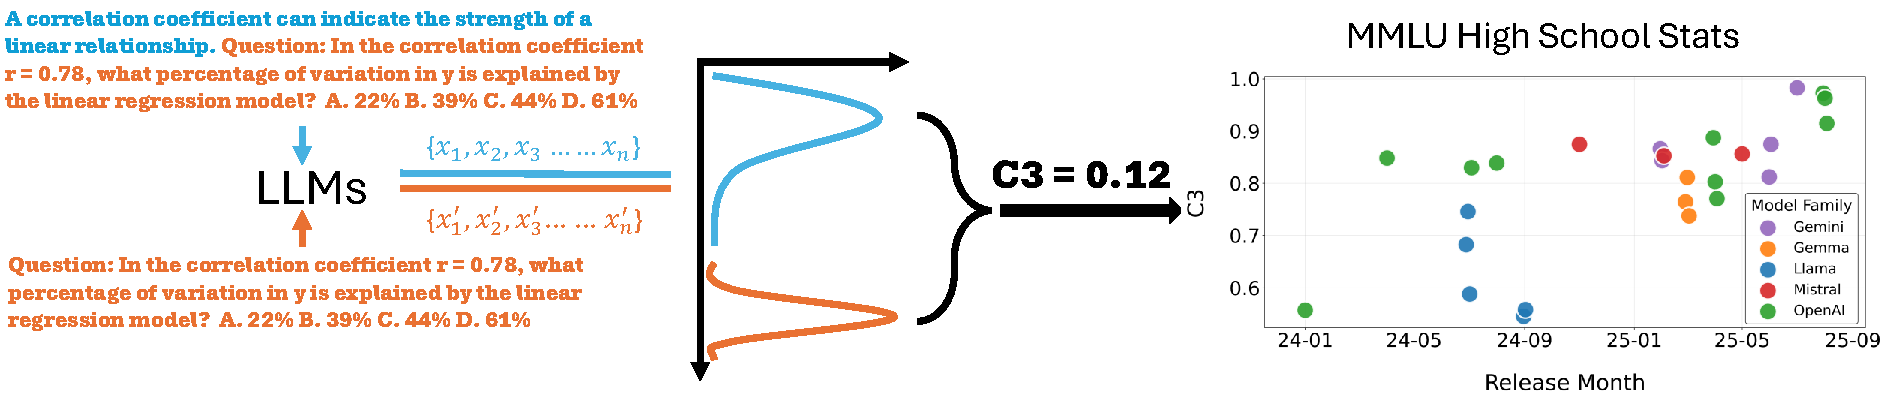
\includegraphics[width=\textwidth]{figure_1.pdf}
    \caption{\revised{C3 workflow. Generations from the unchanged original task are compared with generations after a contextual premise is prefixed. The historical model panel summarizes the existing 26-model MMLU High School Statistics case study; changes across release dates are descriptive associations, not evidence that release date causes greater credibility.}}
    \label{fig:workflow}
\end{figure*}

\begin{revision}
\section{Cross-Contextual Consistency}
\label{sec:c3}
\subsection{Behavioral hypothesis and scope}
\label{sec:logic}
Relevant knowledge may constrain an answer across contexts that provide no new evidence about it. This motivates the hypothesis that contextual stability is associated with answer support. It is not an equivalence: memorization, stable misconceptions, or shortcuts can also yield stable answers. Conversely, low stability need not imply missing knowledge. We test behavioral predictions of this hypothesis rather than estimate a probability of logical entailment or recover the model's internal reasoning process.

\subsection{The contextual intervention}
For an original prompt $x$, let $\mathcal E=\{\epsilon_1,\ldots,\epsilon_L\}$ be a set of generated premises. The evaluated prompt is $x_\epsilon=[\epsilon;x]$, with $x$ copied unchanged. A premise should satisfy three requirements. \textbf{Topic alignment} means remaining in the task's broad domain or capability. \textbf{Answer neutrality} means neither revealing, supporting, contradicting, nor changing the requested answer or judgment. \textbf{Contextual diversity} means adding non-duplicate context rather than rewriting the question. Neutrality is a task-semantic requirement; it does not require invariant model representations, which would prevent the very behavior we aim to measure.

GPT-4.1 generates short premises using the instructions in Appendix~\ref{app:prompt for sampling}. An MPNet embedding filter removes near-duplicate premises at cosine similarity threshold $0.8124$. Paraphrases of auxiliary premises were used only to choose this redundancy threshold (Appendix~\ref{app:diversity of noise}); evaluated questions are not paraphrased by C3. Prompt constraints and filtering do not guarantee neutrality, so we separately assess the generated material (Section~\ref{sec:neutrality}).

\subsection{Sampling and scoring}
We sample $\mathcal Y=\{y_i\}_{i=1}^{n}$ from $P(Y\mid x)$ and $\mathcal Z=\{z_j\}_{j=1}^{m}$ under the contextual conditions, approximating
\begin{equation}
 P^{\mathcal E}(Y\mid x)=\frac{1}{L}\sum_{\epsilon\in\mathcal E}P(Y\mid[\epsilon;x]).
\end{equation}
This compares the original distribution with a mixture over premises. Opposing premise-specific shifts can cancel in the mixture; the pooled score is not a guarantee of invariance to every premise.

Given an answer-similarity kernel $k$, a distributional implementation uses the unbiased squared Maximum Mean Discrepancy (MMD) estimator~\citep{JMLR:v13:gretton12a}:
\begin{equation}
\begin{aligned}
 \widehat D_U={}&\frac{\sum_{i\ne i'}k(y_i,y_{i'})}{n(n-1)}\\
 &+\frac{\sum_{j\ne j'}k(z_j,z_{j'})}{m(m-1)}
 -\frac{2\sum_{i,j}k(y_i,z_j)}{nm}.
\end{aligned}
\label{eq:mmd_main}
\end{equation}
For the indicator kernel used in the new categorical analyses, the reported score is
\begin{equation}
 C_{\mathrm{MMD}}=1-\operatorname{clip}(\widehat D_U/2,0,1).
\label{eq:c3_mmd}
\end{equation}
Clipping handles negative finite-sample unbiased estimates. The score is a stability statistic, not a fitted probability of correctness.

We also report the cross-comparison agreement score
\begin{equation}
 C_{\mathrm{cross}}=\frac{1}{nm}\sum_{i,j}k(y_i,z_j).
\label{eq:c3_cross}
\end{equation}
For categorical answers with frequencies $p$ and $q$, indicator-kernel population MMD is $\sum_c(p_c-q_c)^2$, whereas $C_{\mathrm{cross}}=\sum_c p_cq_c$. Cross-comparison depends on concentration as well as agreement between conditions. For example, identical uniform binary distributions have zero population MMD but cross-comparison $1/2$. Total-variation stability, $C_{\mathrm{TV}}=1-\frac12\sum_c|p_c-q_c|$, is a third, distinct statistic. These distinctions matter in the opinion experiment.

\paragraph{Answer representation and cost.}
Categorical outputs use normalized extracted answers and an equality kernel. Open-ended comparisons may use embeddings or an equivalence judge; these choices require their own validation and do not automatically meet the assumptions of a characteristic kernel. MMD uses within-condition and cross-condition comparisons, while cross-comparison uses only the latter. Direct pairwise implementations cost $O(n^2+m^2+nm)$ and $O(nm)$, respectively; both are quadratic when $m=n$. Categorical frequency counts avoid explicit pair enumeration. Runtime claims must also account for generation, extraction, and judging. Appendix~\ref{app:Operationalization through MMD} distinguishes the implementations found in the experiment records.
\end{revision}

\begin{revision}
\section{Experimental setup}
\paragraph{Original evaluation.}
The original study evaluates SVAMP, MMLU High School Statistics, CommonsenseQA, SimpleQA Verified, FActScore, and HumanEval~\citep{patel-etal-2021-nlp,hendryckstest2021,talmor-etal-2019-commonsenseqa,haas2025simpleqaverifiedreliablefactuality,min-etal-2023-factscore,DBLP:journals/corr/abs-2107-03374}. It reports 16 main models, 30 generations per original and perturbed condition, and 10 additional models in the MMLU case study. Baselines are self-reported confidence, self-consistency, and paraphrasing consistency. FActScore supplies an external factual-support evaluation for long-form text, rather than a comparable reference-free confidence row in Table~\ref{tab:main_results}. Model and benchmark details appear in Appendices~\ref{app:Models} and~\ref{app:benchmark_details_prompts}.

\paragraph{Additional studies.}
The completed FreshQA run uses 50 questions, four models, and 20 samples in each of four conditions (Section~\ref{sec:cutoff}). TopicMisinfo uses 50 sampled claims and 14 models with 20 responses per condition (Section~\ref{sec:opinion}). These smaller studies have separate protocols and are not additional 16-model benchmark blocks. The human neutrality audit concerns 100 MMLU perturbations judged by three annotators.

\paragraph{Quality and calibration.}
We report ECE, AUROC, and precision--recall measures for positive and negative labels (AUPRC-P/N). In the original evaluation, ECE compares scores with mean generation performance; ranking labels threshold that performance at $0.5$. TopicMisinfo instead uses a binary label for proximity to an annotator reference. Scores are evaluated on their stated scales without a fitted calibration map. Lower ECE in these settings does not by itself establish a universally calibrated correctness probability. Appendix~\ref{app:Evaluation Metrics} specifies the targets.

\paragraph{Answer comparison.}
The original study describes Qwen3-8B at temperature zero for large-scale equivalence judgments~\citep{qwen3technicalreport}, using vLLM on two H200 GPUs~\citep{kwon2023efficient}. An equivalence decision concerns substantive answer identity rather than correctness, but can still introduce errors. FreshQA uses cached core-answer extraction followed by target-blind normalization; TopicMisinfo uses deterministic rating extraction. The exact comparison path must be distinguished by task. Appendix~\ref{app:revision_audit} records remaining provenance checks.
\end{revision}

\begin{table*}[t]
\centering

\scriptsize
\setlength{\tabcolsep}{2pt}
\renewcommand{\arraystretch}{1.3}

\begin{tabular*}{\linewidth}{@{\extracolsep{\fill}} l | cccc | cccc @{}}
\toprule 
& \multicolumn{4}{c|}{\textbf{CommonsenseQA}} & \multicolumn{4}{c}{\textbf{SVAMP}} \\
\textbf{Method}
& \makecell[c]{\scriptsize ECE $\downarrow$}
& \makecell[c]{\scriptsize AUROC $\uparrow$}
& \makecell[c]{\scriptsize AUPRC-P $\uparrow$}
& \makecell[c]{\scriptsize AUPRC-N $\uparrow$}
& \makecell[c]{\scriptsize ECE $\downarrow$}
& \makecell[c]{\scriptsize AUROC $\uparrow$}
& \makecell[c]{\scriptsize AUPRC-P $\uparrow$}
& \makecell[c]{\scriptsize AUPRC-N $\uparrow$} \\
\midrule
Self-consistency
& 0.224  &0.643    &0.756    &0.461
& 0.142  &0.861    &0.893    &0.740 \\
Paraphrasing
& 0.271  &0.634    &0.764    &0.484
& 0.157  &0.841    &0.873    &0.720 \\
Self-report
& 0.191  &0.542    &0.746    &0.332
& 0.240  &0.532    &0.763    &0.277 \\

C3 (Ours)
& \cellcolor{gray!20}0.189  & \cellcolor{gray!20} 0.722  & \cellcolor{gray!20}0.805 & \cellcolor{gray!20}0.541
& \cellcolor{gray!20}0.072 & \cellcolor{gray!20}0.917 & \cellcolor{gray!20}0.936 & \cellcolor{gray!20}0.818 \\
\midrule
\midrule
& \multicolumn{4}{c|}{\textbf{MMLU High School Statistics}} & \multicolumn{4}{c}{\textbf{FActScore}} \\
\textbf{Method}
& \makecell[c]{\scriptsize ECE $\downarrow$}
& \makecell[c]{\scriptsize AUROC $\uparrow$}
& \makecell[c]{\scriptsize AUPRC-P $\uparrow$}
& \makecell[c]{\scriptsize AUPRC-N $\uparrow$}
& \makecell[c]{\scriptsize ECE $\downarrow$}
& \makecell[c]{\scriptsize AUROC $\uparrow$}
& \makecell[c]{\scriptsize AUPRC-P $\uparrow$}
& \makecell[c]{\scriptsize AUPRC-N $\uparrow$} \\
\midrule
Self-consistency
& 0.382  &0.577    &0.511    &0.605
& 0.225  &0.858    &0.909    &\cellcolor{gray!20}0.731 \\
Paraphrasing
& 0.406  &0.547    &0.489    &0.591
& 0.249  &0.828    &0.887    &0.716 \\
Self-report
&  0.378  &0.496    &\cellcolor{gray!20}0.594    &0.411
& 0.330  &0.496    &0.706    &0.335 \\
C3 (Ours)
& \cellcolor{gray!20}0.338 &\cellcolor{gray!20}0.597    &0.530    &\cellcolor{gray!20}0.621
&\cellcolor{gray!20} 0.160  &\cellcolor{gray!20}0.873    &\cellcolor{gray!20}0.916    &0.701 \\
\midrule
\midrule
& \multicolumn{4}{c|}{\textbf{HumanEval}} & \multicolumn{4}{c}{\textbf{SimpleQA}} \\
\textbf{Method}
& \makecell[c]{\scriptsize ECE $\downarrow$}
& \makecell[c]{\scriptsize AUROC $\uparrow$}
& \makecell[c]{\scriptsize AUPRC-P $\uparrow$}
& \makecell[c]{\scriptsize AUPRC-N $\uparrow$}
& \makecell[c]{\scriptsize ECE $\downarrow$}
& \makecell[c]{\scriptsize AUROC $\uparrow$}
& \makecell[c]{\scriptsize AUPRC-P $\uparrow$}
& \makecell[c]{\scriptsize AUPRC-N $\uparrow$} \\
\midrule
Self-consistency
& 0.131  &0.812    &0.896    &0.487
& 0.393  &0.792    &0.368    &0.924 \\
Paraphrasing
& 0.165  &0.778    &0.862   &0.453
& 0.411  &0.773    &0.349    &0.906 \\
Self-report
& 0.287  &0.528    &0.807    &0.211
& 0.778 & 0.490 &  0.151  & 0.846 \\

C3 (Ours)
& \cellcolor{gray!20}0.110 & \cellcolor{gray!20}0.847 & \cellcolor{gray!20}0.943 & \cellcolor{gray!20}0.520
& \cellcolor{gray!20}0.166 & \cellcolor{gray!20}0.823 & \cellcolor{gray!20}0.389 & \cellcolor{gray!20}0.944 \\
\bottomrule
\end{tabular*}

\caption{\revised{Original six-benchmark results, reported as averages over 16 models. Numerical entries are retained from the source manuscript. Shading indicates the best reported value within each benchmark and metric. ECE is lower-is-better; the ranking metrics are higher-is-better. The added FreshQA and TopicMisinfo studies are reported separately with explicit estimator names and sample counts. Appendix~\ref{app:revision_audit} identifies the remaining provenance checks for the original score implementations.}}
\label{tab:main_results}
\end{table*}

\begin{revision}
\section{Results}
\subsection{Predicting task-specific answer quality}
Table~\ref{tab:main_results} retains the original aggregate comparisons. C3 has higher reported AUROC than the three baselines across all six benchmarks, including $0.917$ versus $0.861$ for self-consistency on SVAMP and $0.823$ versus $0.792$ on SimpleQA. Gains are not uniform across metrics: self-reported confidence has higher AUPRC-P on MMLU, and self-consistency has higher AUPRC-N on FActScore. These comparisons support predictive utility in the tested settings, without showing that C3 recovers the logical coherence or internal grounding of individual answers.

On FActScore, C3's reported ECE and AUROC are $0.160$ and $0.873$. FActScore evaluates atomic claims against external evidence, whereas C3 probes response behavior. Their association supports a retrieval-free diagnostic at scoring time, not replacement of factual verification. Auxiliary premise generation and answer comparison still incur costs. Extended scaling and factuality plots are retained in Appendix~\ref{app:extended_results}.
\end{revision}

\begin{revision}
\subsection{Validation of contextual premises}
\label{sec:neutrality}
The existing MMLU analysis compares the number of correct responses among 30 original and 30 perturbed generations for each model--question pair. Its approximately zero-centered differences provide a check for aggregate directional effects, not instance-level neutrality. A separate domain-classification check assigns approximately $96\%$ of premises to the intended benchmark domain; it assesses topic alignment rather than answer relevance.

In an additional human study, all three annotators independently assessed each of 100 MMLU perturbations alongside its question and correct answer. They judged whether the added context helped, was neutral, or hurt the answer. Ninety-four perturbations were unanimously judged neutral. This is evidence about the inspected sample under a strict agreement criterion, not a guarantee for every premise, task, or model. The remaining six items cannot be characterized without their individual judgments. Appendix~\ref{app:human_neutrality} gives the supplied protocol and flags the records needed to complete this audit.
\end{revision}

\begin{revision}
\subsection{Knowledge cutoff and contextual stability}
\label{sec:cutoff}
We analyze a matched FreshQA subset~\citep{vu-etal-2024-freshllms} containing 25 facts established by 2022 and 25 facts first established in 2025. Four models with documented cutoffs no later than August 2024 are evaluated: GPT-4.1, GPT-4.1 mini, Gemma 3 27B, and Llama 3.1 70B. The completed run samples 20 responses in each of four arms: two independent original-prompt replicates, surface-format variants, and contextual premises. The reference date is fixed across arms. Each control is compared with the same original replicate using the same estimator; original-replicate MMD is a sampling control, not within-prompt answer concentration.
\end{revision}


\begin{table}[t]
\centering\small\revisioncolor
\setlength{\tabcolsep}{3pt}
\begin{tabular}{lrr}
\toprule
Diagnostic & Pre-cutoff & Post-cutoff\\
\midrule
Original accuracy & .659 & .126\\
\midrule
MMD: original replicates & .999 & .994\\
MMD: format & .984 & .980\\
MMD: context & .976 & .946\\
\midrule
Cross: original replicates & .812 & .579\\
Cross: format & .786 & .537\\
Cross: context & .771 & .469\\
\bottomrule
\end{tabular}
\caption{FreshQA means across four models and 25 questions per cutoff group. MMD and cross-comparison are reported on separate scales. Matched-pair bootstrap intervals and model-level results appear in Appendix~\ref{app:freshqa}.}
\label{tab:freshqa}
\end{table}
\begin{revision}
Accuracy is lower for post-cutoff facts (Table~\ref{tab:freshqa}), supporting the intended difference in plausible knowledge availability. MMD contextual stability decreases by $0.030$ (matched-pair cluster-bootstrap 95\% CI $[0.006,0.054]$), while the format-only decrease is $0.004$ ($[-0.011,0.019]$). Contextual distance exceeds format distance by $0.021$ ($[0.011,0.032]$), averaged over both groups. However, the post-minus-pre increase in this excess distance is $0.026$, with a two-sided interval of $[-0.002,0.052]$. Thus, the specific cutoff-by-condition interaction is less certain than the contextual contrast overall.

Cross-comparison shows a larger decline, from $0.771$ to $0.469$, but original-replicate and format agreement also decline substantially. This quantity includes answer concentration, so its full decrease cannot be attributed to contextual distributional shift. Its excess context-versus-format distance increases by $0.052$ ($[0.009,0.094]$). Together, the controls support a behavioral association with the cutoff grouping while leaving temporal content differences, stable errors, and the internal basis of responses unresolved.
\end{revision}

\begin{revision}
\subsection{Alignment with human opinion ratings}
\label{sec:opinion}
TopicMisinfo~\citep{neumann2026opinions} contains human judgments of the potential harm of claims to demographic groups. We evaluate a topic-stratified sample of 50 claims with 14 models, asking for a six-point rating from the perspective of a statistically average person. The human reference equally weights the mean ratings of male and female annotators. A model--claim pair is labeled aligned when the original-prompt mean rating is within one point of that reference. After requiring complete response slots and at least five extracted ratings per condition, 663 pairs remain, with 34--50 claims per model. This measures alignment with the dataset's annotator reference, not factual truth or population representativeness.
\end{revision}


\begin{table*}[t]
\centering\small\revisioncolor
\begin{tabular}{lrrrr}
\toprule
Score & ECE $\downarrow$ & AUROC $\uparrow$ & AUPRC-P $\uparrow$ & AUPRC-N $\uparrow$\\
\midrule
Self-consistency (plurality) & 0.213 & 0.700 & 0.741 & 0.610 \\
Same-prompt pairwise agreement & 0.179 & 0.716 & 0.759 & 0.618 \\
Same-prompt concentration & 0.187 & 0.718 & 0.766 & 0.617 \\
C3 (MMD) & 0.421 & 0.554 & 0.593 & 0.539 \\
C3 (total variation) & 0.277 & 0.638 & 0.696 & 0.574 \\
C3 (cross-comparison) & 0.164 & 0.712 & 0.764 & 0.613 \\

\bottomrule
\end{tabular}
\caption{TopicMisinfo macro averages over 14 models, recomputed from cached responses on the same retained instances within each model. All methods use 20 original response slots; contextual scores also use 20 perturbed slots. Same-prompt concentration is one minus categorical entropy normalized by $\log 6$. These are descriptive comparisons without a fitted score-calibration map.}
\label{tab:topicmisinfo}
\end{table*}
\begin{revision}
Cross-comparison improves ECE from $0.213$ to $0.164$ relative to plurality-based self-consistency and raises AUROC from $0.700$ to $0.712$ (Table~\ref{tab:topicmisinfo}). The interpretation is estimator-dependent: MMD and total-variation stability perform worse, while same-prompt pairwise agreement and entropy-based concentration have slightly higher AUROC than cross-comparison. On the 25 claims retained for every model, the ECE advantage remains, but the same-prompt ranking controls again remain competitive (Appendix~\ref{app:topicmisinfo}). Accordingly, this experiment supports the usefulness of contextual agreement on this task, not uniform superiority of distributional stability or a general endorsement of simulated opinions.
\end{revision}

\begin{revision}
\subsection{Implementation sensitivity and benchmark diagnosis}
The original source ablation includes GPT-4.1 premises, Qwen3-8B premises, and web snippets (Appendix~\ref{app:Ablation Study on Source of Noises}). The reported results suggest that useful signals can persist across sources, but changing the source also changes relevance, diversity, and possible answer leakage. This comparison does not isolate the contribution of each perturbation constraint. Likewise, the SimpleQA comparison trades calibration and ranking performance between score implementations (Appendix~\ref{app:Ablation Study on MMD}); it does not establish estimator interchangeability, as the opinion results demonstrate.

Jointly plotting performance and C3 provides a descriptive benchmark diagnostic (Figure~\ref{fig:Effect_analysis}). Correct-but-fragile instances differ from consistently correct ones, and stable incorrect answers differ from unstable errors. These regions identify behaviors worth investigating. They do not independently demonstrate contamination, overfitting, misconceptions, or genuine understanding. Median-based boundaries are relative to the evaluated models and benchmarks, rather than universal thresholds for credibility.
\end{revision}

\begin{figure}[t]

    \centering
    \includegraphics[width=\linewidth]{Bench_diagnosis.png}
    \caption{\revised{Joint performance and contextual-stability diagnostic from the original evaluation, averaged over 16 models. The existing figure uses median splits across six benchmarks. Its labels ``mastered, ``brittle, ``biased, and ``unlearned denote descriptive quadrants only: high/high, high/low, low/high, and low/low performance/stability. They do not establish a learning mechanism, contamination, or demographic bias.}}
    \label{fig:Effect_analysis}

\end{figure}

\begin{revision}
\section{Related work}
\label{Related work}
\paragraph{Same-prompt uncertainty.}
Self-consistency uses repeated generations from one prompt~\citep{DBLP:conf/iclr/0002WSLCNCZ23}; semantic uncertainty groups responses by meaning before estimating uncertainty~\citep{kuhn2023semantic,farquhar2024semantic}. Likelihood-weighted implementations use model scoring access, while empirical-frequency variants can operate on samples. C3's conceptual distinction is access to a second, contextually perturbed distribution, rather than an exclusive ability to support black-box evaluation.

\paragraph{Prompt variation.}
Self-Para-Consistency generates question paraphrases and selects a consistent answer~\citep{chen-etal-2024-self-para}. Code-validation work also uses prompt paraphrases and cross-program testing~\citep{wang2026paraphrasing}. Scenario-independent uncertainty estimation uses factor analysis across scenarios~\citep{wen2025scenario}. These approaches motivate direct comparisons under matched generation budgets. C3 specifies an unchanged task and added answer-neutral context, but shares the broader goal of learning from response variation. SPUQ likewise samples outputs under input perturbations and aggregates their variation to quantify uncertainty~\citep{gao-etal-2024-spuq}.

\paragraph{External verification and opinion simulation.}
FActScore measures the fraction of atomic claims supported by a knowledge source~\citep{min-etal-2023-factscore}; C3 measures behavior without retrieving factual evidence during score computation. These signals answer different questions. For opinion simulation, \citet{neumann2026opinions} evaluate logical consistency and stakeholder alignment. Our extension instead predicts proximity to a particular human-reference rating from contextual response behavior, and does not replace their broader quality checks.
\end{revision}

\begin{revision}
\section{Conclusion}
C3 evaluates how generated answers respond to added context while preserving the original task. The expanded evidence links this intervention to task-specific quality and cutoff-group differences, while exposing important boundaries: stable errors remain possible, neutrality requires validation, and distributional stability can perform differently from cross-comparison agreement. Reporting these distinctions makes contextual probing a complementary behavioral diagnostic rather than a certificate of truthfulness or an identification of internal reasoning.

\section*{Limitations}
Neutrality is an operational design objective, not an intrinsic guarantee. Human validation covers a small MMLU sample, and aggregate accuracy differences can mask opposing effects. Averaging responses across premises can also conceal premise-specific shifts. A factorial ablation of the perturbation constraints and a task-stratified human audit of answer-equivalence judgments remain needed. Auxiliary generation, extraction, and judging can introduce bias and substantial cost even though the evaluated model is accessed through outputs alone.

The cutoff experiment compares matched questions about different facts and dates; it does not directly intervene on model memory. Documented cutoffs neither guarantee acquisition of older facts nor preclude inference of newer answers. Its MMD interaction estimate remains uncertain. The TopicMisinfo extension is limited to 50 claims and a particular annotator reference, excludes insufficiently parsed responses, and finds no uniform advantage over stronger same-prompt controls. Score scaling affects ECE; no universal probability calibration is established. Original benchmark tables are retained pending completion of the implementation and aggregation provenance checks in Appendix~\ref{app:revision_audit}.

\section*{Ethical considerations}
Contextual stability should not be used as a guarantee of truth, safety, or suitability for high-stakes decisions. Consistent errors and demographic stereotypes can persist across contexts. TopicMisinfo ratings characterize alignment with an annotator sample and do not justify replacing affected communities or human participants with LLMs. Human-annotation documentation, including the applicable consent, compensation, and review arrangements, must accompany the neutrality records; no institutional approval or exemption is asserted here without documentation.
\end{revision}

\bibliographystyle{acl_natbib}
\bibliography{citation}
\clearpage
\appendix

\section{Discussion on Perturbation Noise source}\label{app:Discussion on Perturbation Noise source}


\subsection{LLMs as Sampler of Noise}\label{app:LLMs as Sampler of Noise}


We utilize LLMs as samplers to generate semantic perturbations. The noise generation process adheres to three critical principles to ensure the resulting samples are both challenging and informative:

\begin{itemize}
    \item \textbf{Topic Alignment:} Samples are generated to remain semantically aligned with the original input query to ensure the underlying task remains constant.
    \item \textbf{Content Neutrality:} The samples are designed to be content-neutral, as non-neutral content could introduce systematic bias or shifts in the model's performance.
    \item \textbf{Non-Trivial Contextual Variations:} The generated noise constitutes non-trivial contextual variations of the input, testing the model's robustness while maintaining the core meaning.
\end{itemize}

we employ the prompts detailed in Appendix~\ref{app:prompt for sampling}. By utilizing LLMs as samplers constrained by these principles, 
we collect a set of perturbations $\mathcal{E} = \{\epsilon_1, \dots, \epsilon_n\}$. 
To ensure the diversity of $\mathcal{E}$, we filter out candidate noise that is semantically redundant with existing entries (details are provided in Appendix~\ref{app:diversity of noise}).

\begin{revision}
\subsection{Redundancy filtering and auxiliary paraphrases}
\label{app:diversity of noise}
The generator maintains a pool of premises and rejects candidates whose MPNet cosine similarity to an accepted premise exceeds the threshold~\citep{song2020mpnet}. To choose the threshold, the original calibration used 30 generated premises and 50 paraphrases of each, yielding within-premise pairwise similarities. The empirical fifth percentile was $0.8124$ (Figure~\ref{fig:rewrite distribution}). These paraphrases concern auxiliary premises, not the evaluation questions, and are not C3 test inputs.

This threshold is a redundancy heuristic. A tail probability conditional on sampled paraphrases does not determine the probability that an accepted premise is redundant, and it does not validate answer neutrality. No claim of a 5\% false-discovery bound follows from the calibration. The paraphrasing baseline is a separate evaluation procedure that rewrites questions.
\end{revision}

\begin{figure*}[t] 
    \centering
    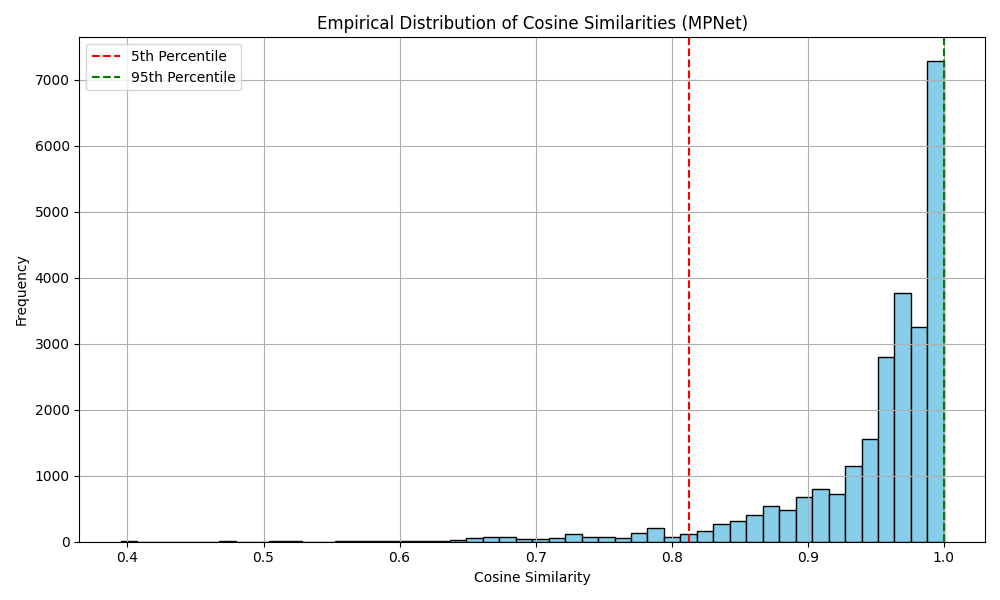
\includegraphics[width=\textwidth]{rewrite_similarity_histogram.png}
    \caption{\revised{Auxiliary premise-paraphrase cosine similarities used to choose a redundancy-filter threshold. The fifth percentile is $0.8124$. This heuristic does not bound the proportion of redundant premises accepted by the filter.}}
    \label{fig:rewrite distribution}
\end{figure*}

\subsection{Semantic Neutrality of Perturbations}
\label{app:semantic neutrality}

Figure~\ref{fig:neutrality} evaluates whether our sampled perturbations introduce systematic answer-relevant bias. We conduct this check on MMLU High School Statistics across 26 models. For each model-question pair, we sample 30 generations from the original prompt and 30 generations from the perturbed prompt. We then compute:
\[
\Delta = \#\text{Correct}_{\text{perturbed}} - \#\text{Correct}_{\text{original}},
\]
where positive values indicate that the perturbation improves performance and negative values indicate that it hurts performance.

If the added context revealed information about the answer, contradicted the question, or otherwise biased the model toward or away from the correct option, we would expect the distribution of $\Delta$ to shift systematically above or below zero. In contrast, Figure~\ref{fig:neutrality} shows that the distribution is centered near zero across all 26 models, with no consistent positive or negative shift. This suggests that the perturbations do not systematically help or mislead the models on this benchmark.

This analysis does not prove that every individual perturbation is perfectly neutral, but it provides empirical evidence that the perturbation procedure does not introduce a systematic directional bias in model performance. We therefore treat these perturbations as approximately content-neutral for the purposes of measuring cross-contextual consistency.
\begin{figure*}[t] 
    \centering
    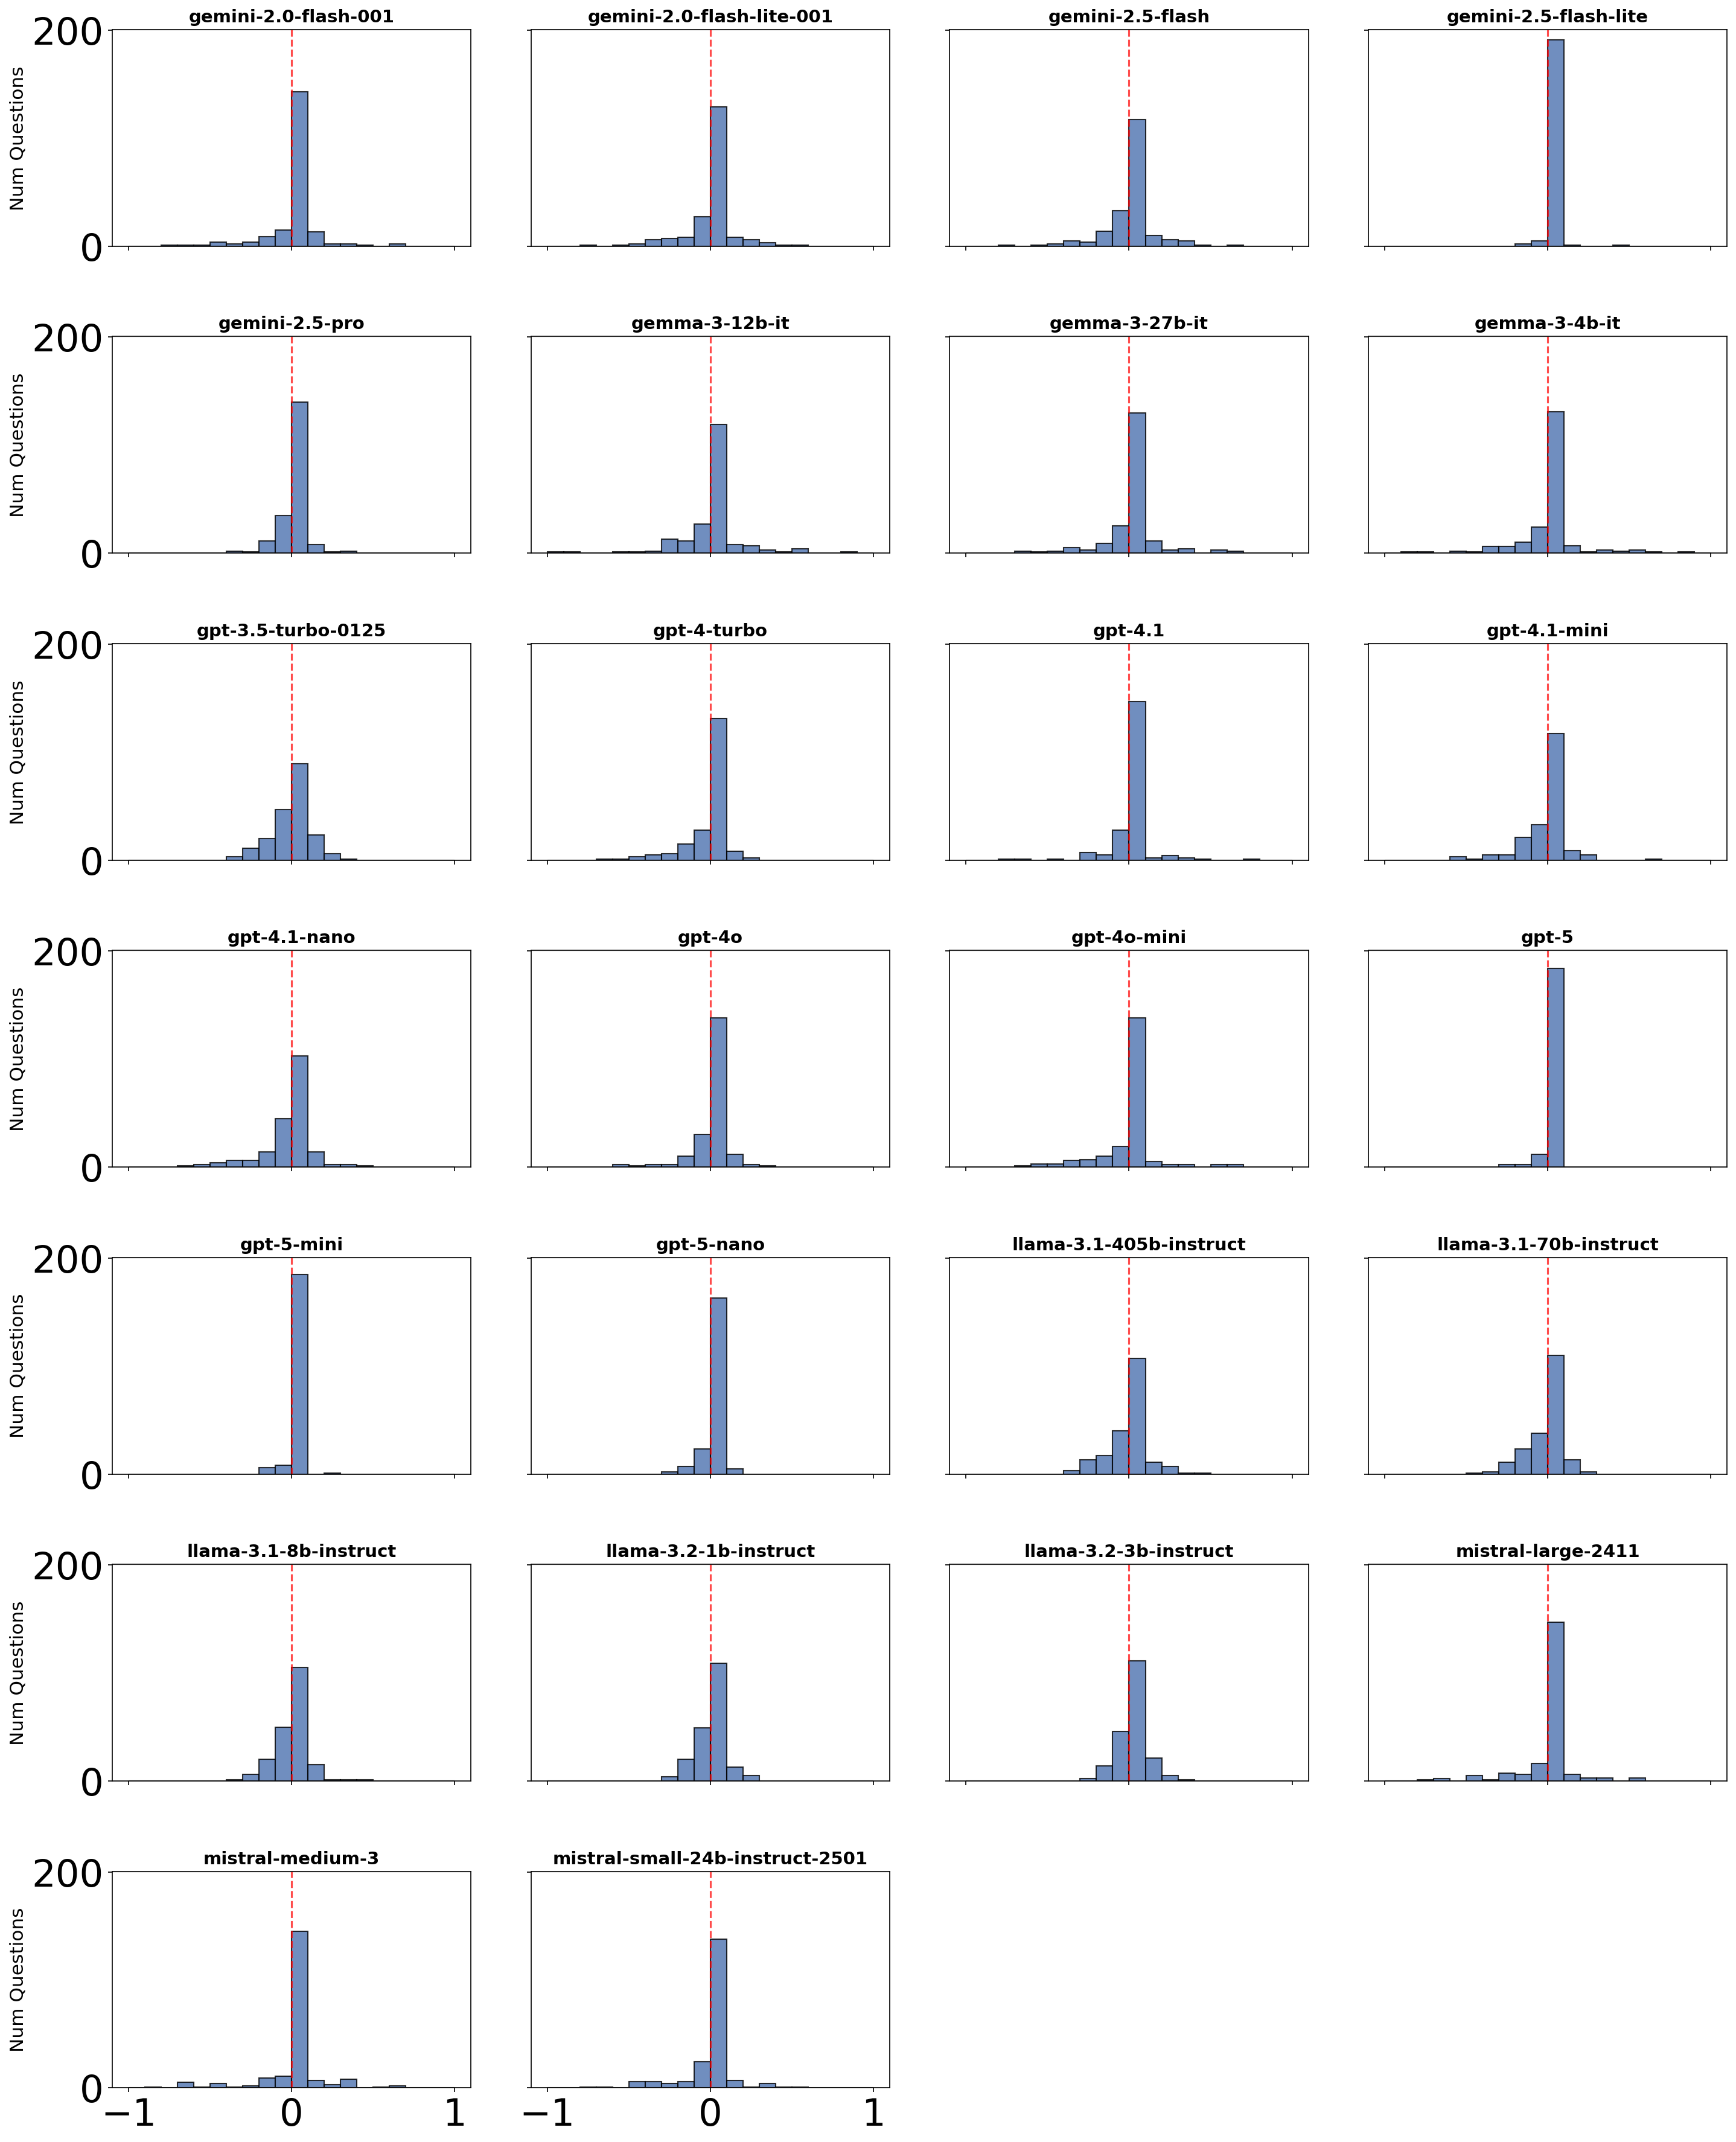
\includegraphics[width=\textwidth]{aggregated_diff_histogram.png}
    \caption{The difference of performance of each model before and after the perturbation noises are added. The red line denote the 0 meaning no difference in the performances.}
    \label{fig:neutrality}
\end{figure*}


\subsection{Topic Alignment}
\label{app:Topic Alignment}

We also evaluate whether the sampled perturbations remain topic-aligned with the benchmark from which they are generated. Topic alignment means that the perturbation should stay within the broad domain or capability being tested, without revealing, contradicting, or otherwise modifying the answer. This requirement separates our perturbations from arbitrary distractor text: the added context should create meaningful contextual variation, but should still be relevant to the type of task being evaluated.

To assess topic alignment, we conduct an automatic topic-classification check. For each benchmark, we used whole perturbations generated by our pipeline with GPT-4.1 and remove the corresponding original question and answer. We then ask an independent Qwen3-8B judge to classify each perturbation into one of the broad benchmark-level domains: arithmetic reasoning, statistical reasoning, commonsense reasoning, short-form factual recall, long-form factual or biographical generation, and code generation. The judge observes only the perturbation itself, not the original query, answer, or benchmark label. A perturbation is counted as topic-aligned if the judge assigns it to the same broad domain as the benchmark from which it was sampled.

Across the perturbations, approximately 96\% are classified into their intended benchmark domain. This suggests that the perturbations are not arbitrary out-of-domain distractors but instead remain aligned with the capability being evaluated. Together with the neutrality analysis in Appendix~\ref{app:semantic neutrality}, this supports the use of our sampled perturbations as topic-aligned, answer-neutral contextual variations for estimating cross-contextual consistency.


\section{Empirical Choice of number of trials}\label{app:number of trials}
To choose an appropriate number of trials, we conducted a case study to determine how many samples per question are needed to reliably characterize model behavior before and after perturbation. As shown in Figure~\ref{fig:trial_convergence}, the estimated behavior stabilizes after about 20 samples. We therefore use 30 trials per question as a more conservative choice in this setting.
\begin{figure*}[t] 
    \centering
    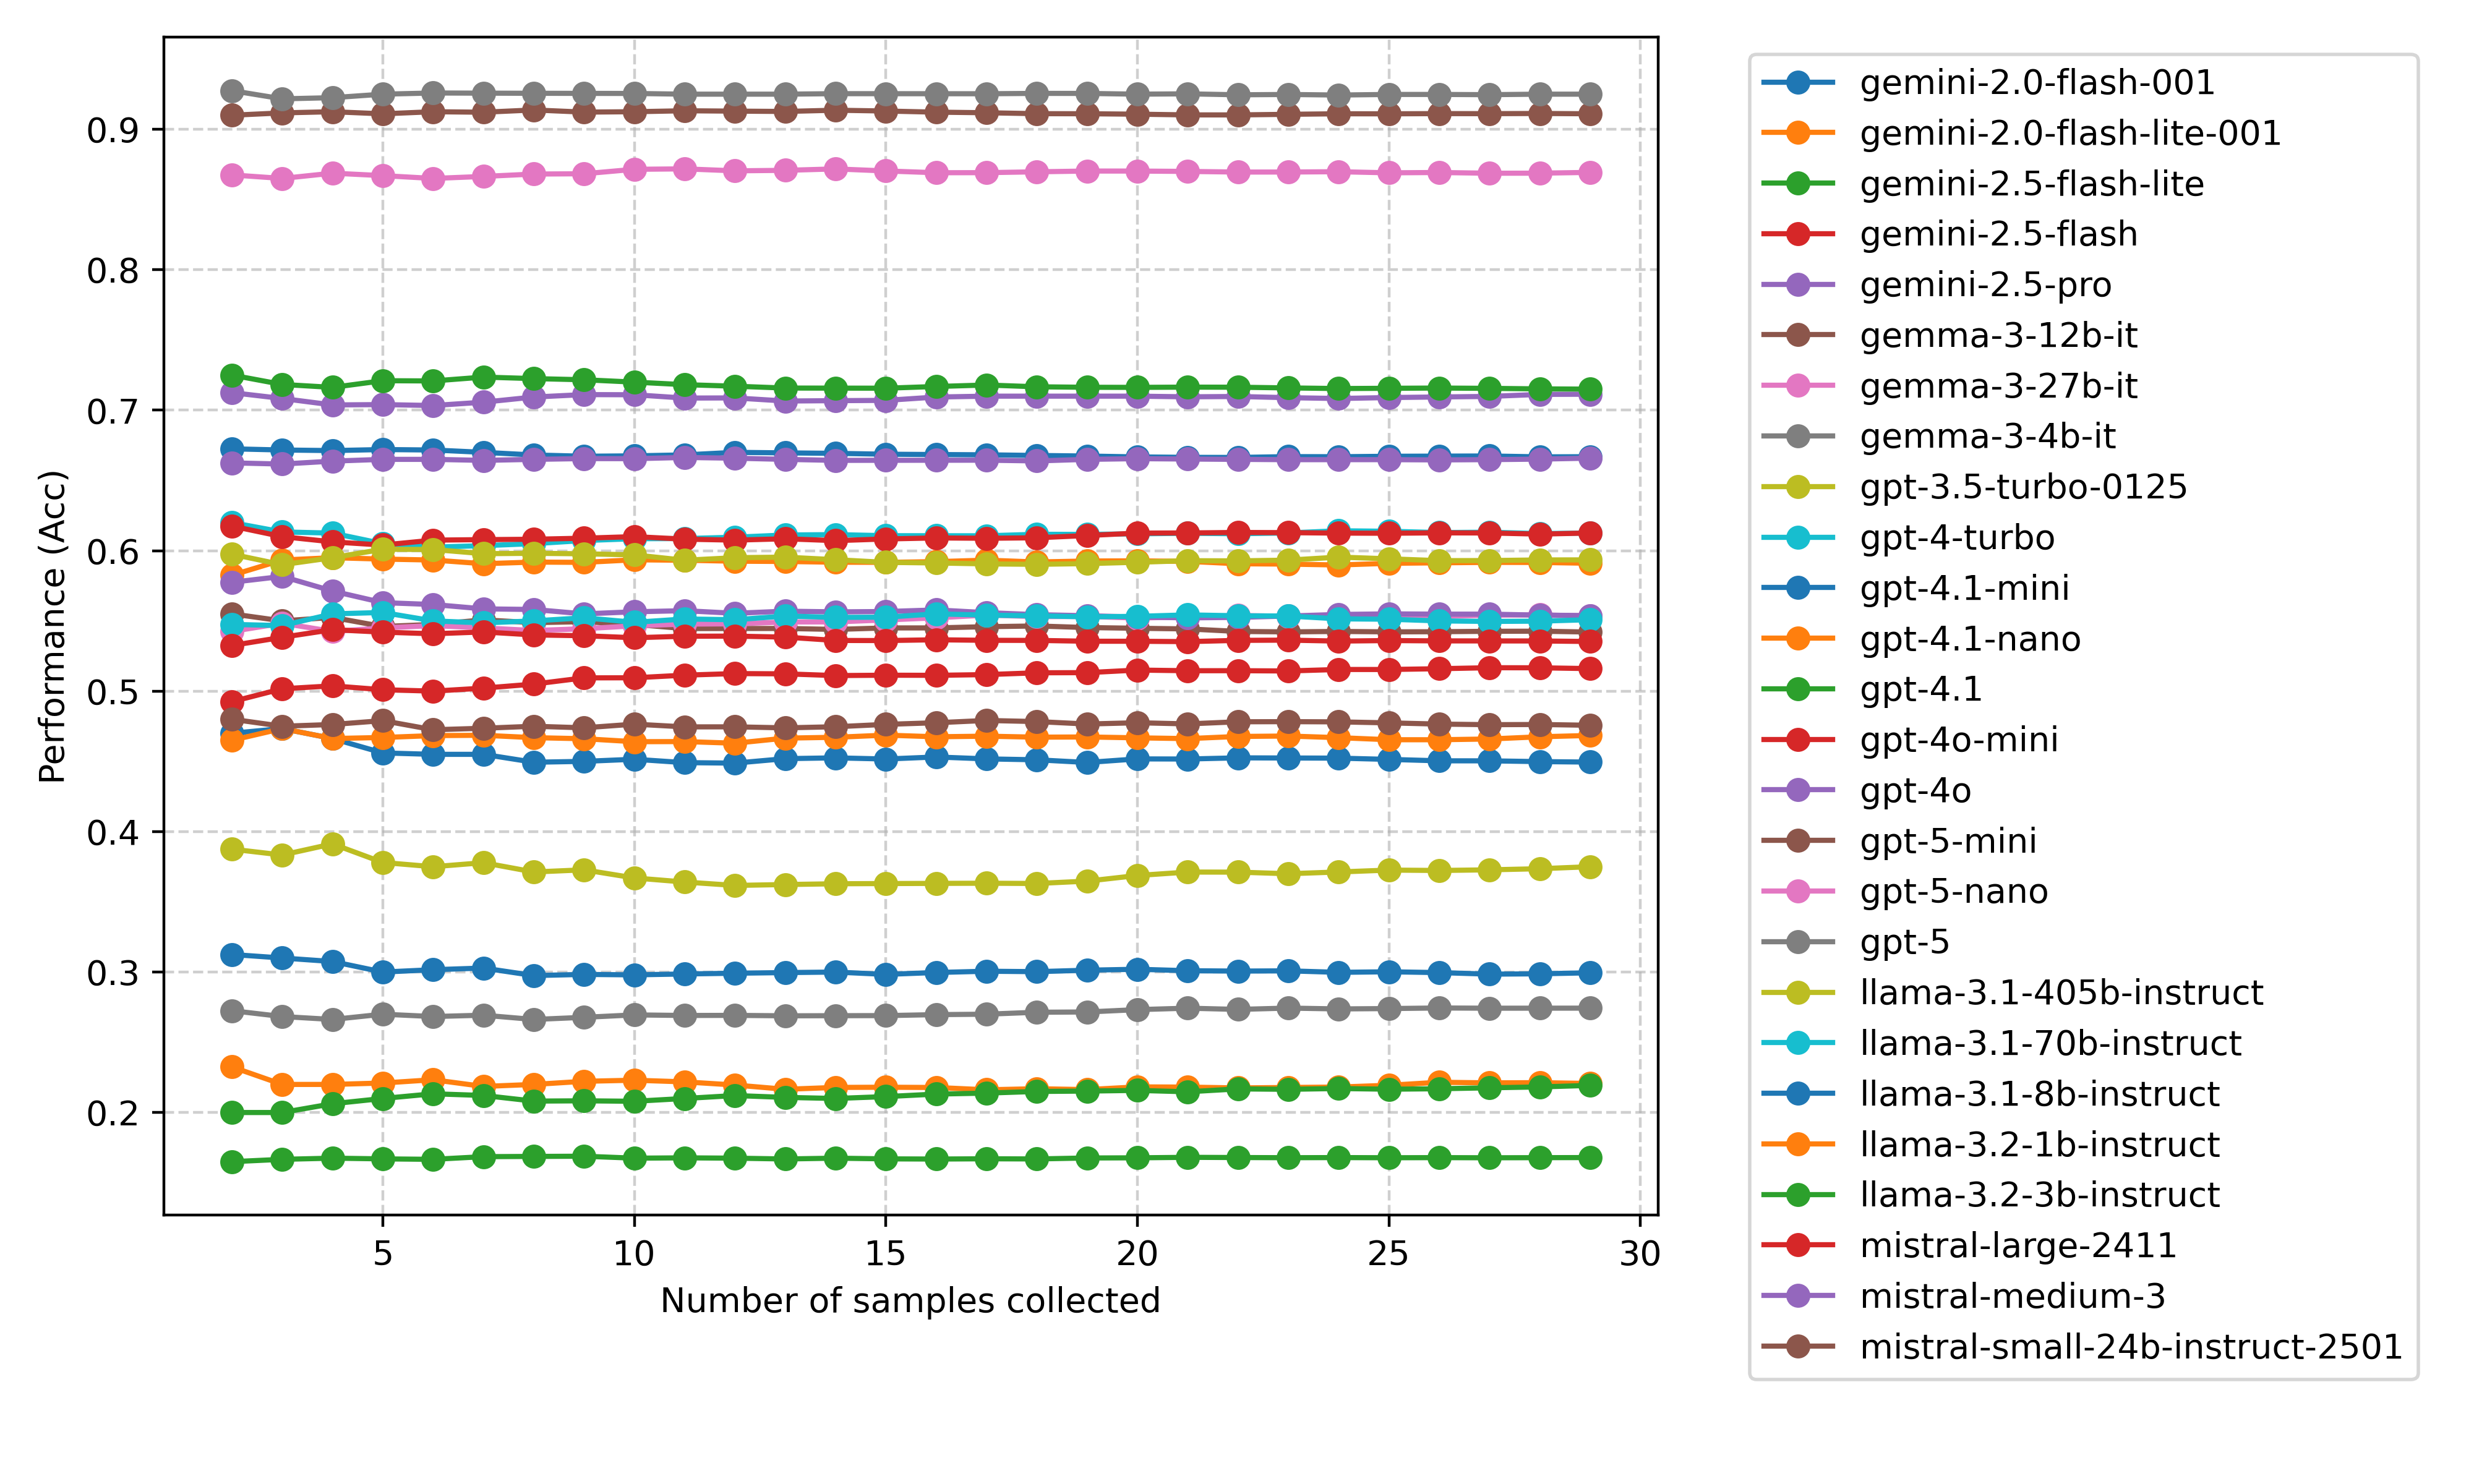
\includegraphics[width=\textwidth]{trial_convergence.png}
    \caption{The performance of models across number of trials of samples we collected when perturbation is presented.}
    \label{fig:trial_convergence}
\end{figure*}


\section{C3 Evaluation on Model-Level}\label{app:model level evaluation}
\begin{table*}[p]
\centering
\caption{MMLU High School Stats Model Performance Metrics}
\label{tab:model-metrics}
\scriptsize % Reduces font size slightly to fit width comfortably
\begin{minipage}[t]{0.48\textwidth}
    \centering
    \begin{tabular}{lcccc}
        \toprule
        \textbf{Metric} & \textbf{ECE} & \textbf{AUROC} & \textbf{PR-P} & \textbf{PR-N} \\
        \midrule
        \multicolumn{5}{l}{\textbf{gemini-2.5-flash}} \\
        self-consistency & 0.359 & 0.506 & 0.527 & 0.495 \\
        Paraphrasing     & 0.394 & 0.456 & 0.452 & 0.472 \\
        C3              & 0.327 & 0.549 & 0.569 & 0.501 \\
        Self-report      & 0.271 & 0.492 & 0.741 & 0.237 \\
        \midrule
        \multicolumn{5}{l}{\textbf{gemini-2.5-flash-lite}} \\
        self-consistency & 0.795 & 0.503 & 0.166 & 0.835 \\
        Paraphrasing     & 0.808 & 0.450 & 0.150 & 0.789 \\
        C3            & 0.818 & 0.523 & 0.172 & 0.848 \\
        Self-report      & 0.374 & 0.519 & 0.579 & 0.442 \\
        \midrule
        \multicolumn{5}{l}{\textbf{gemma-3-12b-it}} \\
        self-consistency & 0.304 & 0.646 & 0.650 & 0.568 \\
        Paraphrasing     & 0.310 & 0.609 & 0.677 & 0.590 \\
        C3            & 0.241 & 0.679 & 0.689 & 0.592 \\
        Self-report      & 0.395 & 0.511 & 0.589 & 0.446 \\
        \midrule
        \multicolumn{5}{l}{\textbf{gemma-3-27b-it}} \\
        self-consistency & 0.326 & 0.647 & 0.663 & 0.543 \\
        Paraphrasing     & 0.329 & 0.608 & 0.660 & 0.555 \\
       C3             & 0.260 & 0.706 & 0.721 & 0.613 \\
        Self-report      & 0.423 & 0.458 & 0.549 & 0.420 \\
        \midrule
        \multicolumn{5}{l}{\textbf{gemma-3-4b-it}} \\
        self-consistency & 0.602 & 0.628 & 0.335 & 0.798 \\
        Paraphrasing     & 0.666 & 0.596 & 0.348 & 0.785 \\
       C3             & 0.504 & 0.595 & 0.324 & 0.776 \\
        Self-report      & 0.530 & 0.496 & 0.307 & 0.716 \\
        \midrule
        \multicolumn{5}{l}{\textbf{gpt-4.1}} \\
        self-consistency & 0.202 & 0.739 & 0.839 & 0.503 \\
        Paraphrasing     & 0.226 & 0.698 & 0.827 & 0.482 \\
       C3             & 0.180 & 0.753 & 0.856 & 0.528 \\
        Self-report      & 0.273 & 0.499 & 0.740 & 0.269 \\
        \midrule
        \multicolumn{5}{l}{\textbf{gpt-4.1-mini}} \\
        self-consistency & 0.416 & 0.536 & 0.493 & 0.561 \\
        Paraphrasing     & 0.418 & 0.506 & 0.494 & 0.506 \\
       C3             & 0.404 & 0.521 & 0.502 & 0.546 \\
        Self-report      & 0.233 & 0.592 & 0.879 & 0.232 \\
        \midrule
        \multicolumn{5}{l}{\textbf{gpt-4.1-nano}} \\
        self-consistency & 0.374 & 0.487 & 0.494 & 0.490 \\
        Paraphrasing     & 0.357 & 0.516 & 0.504 & 0.455 \\
       C3             & 0.358 & 0.493 & 0.510 & 0.502 \\
        Self-report      & 0.367 & 0.480 & 0.644 & 0.332 \\
        \bottomrule
    \end{tabular}
\end{minipage}
\hfill
\begin{minipage}[t]{0.48\textwidth}
    \centering
    \begin{tabular}{lcccc}
        \toprule
        \textbf{Metric} & \textbf{ECE} & \textbf{AUROC} & \textbf{PR-P} & \textbf{PR-N} \\
        \midrule
        \multicolumn{5}{l}{\textbf{llama-3.1-405b-instruct}} \\
        self-consistency & 0.122 & 0.784 & 0.849 & 0.618 \\
        Paraphrasing     & 0.164 & 0.757 & 0.828 & 0.633 \\
       C3             & 0.077 & 0.793 & 0.858 & 0.639 \\
        Self-report      & 0.300 & 0.508 & 0.743 & 0.274 \\
        \midrule
        \multicolumn{5}{l}{\textbf{llama-3.1-70b-instruct}} \\
        self-consistency & 0.211 & 0.598 & 0.657 & 0.500 \\
        Paraphrasing     & 0.209 & 0.536 & 0.617 & 0.523 \\
       C3             & 0.209 & 0.549 & 0.635 & 0.456 \\
        Self-report      & 0.276 & 0.520 & 0.747 & 0.271 \\
        \midrule
        \multicolumn{5}{l}{\textbf{llama-3.1-8b-instruct}} \\
        self-consistency & 0.366 & 0.490 & 0.308 & 0.686 \\
        Paraphrasing     & 0.395 & 0.480 & 0.260 & 0.625 \\
       C3             & 0.285 & 0.494 & 0.308 & 0.700 \\
        Self-report      & 0.489 & 0.491 & 0.373 & 0.632 \\
        \midrule
        \multicolumn{5}{l}{\textbf{llama-3.2-1b-instruct}} \\
        self-consistency & 0.492 & 0.538 & 0.220 & 0.832 \\
        Paraphrasing     & 0.540 & 0.517 & 0.180 & 0.773 \\
       C3             & 0.360 & 0.569 & 0.215 & 0.853 \\
        Self-report      & 0.576 & 0.517 & 0.163 & 0.862 \\
        \midrule
        \multicolumn{5}{l}{\textbf{llama-3.2-3b-instruct}} \\
        self-consistency & 0.470 & 0.477 & 0.192 & 0.814 \\
        Paraphrasing     & 0.476 & 0.480 & 0.198 & 0.759 \\
       C3             & 0.358 & 0.544 & 0.228 & 0.846 \\
        Self-report      & 0.540 & 0.477 & 0.286 & 0.696 \\
        \midrule
        \multicolumn{5}{l}{\textbf{mistral-large-2411}} \\
        self-consistency & 0.371 & 0.484 & 0.548 & 0.433 \\
        Paraphrasing     & 0.432 & 0.424 & 0.507 & 0.423 \\
       C3             & 0.380 & 0.521 & 0.573 & 0.463 \\
        Self-report      & 0.361 & 0.403 & 0.685 & 0.227 \\
        \midrule
        \multicolumn{5}{l}{\textbf{mistral-medium-3}} \\
        self-consistency & 0.286 & 0.629 & 0.731 & 0.445 \\
        Paraphrasing     & 0.317 & 0.600 & 0.654 & 0.493 \\
       C3             & 0.220 & 0.751 & 0.823 & 0.547 \\
        Self-report      & 0.274 & 0.499 & 0.772 & 0.242 \\
        \midrule
        \multicolumn{5}{l}{\textbf{mistral-small-24b}} \\
        self-consistency & 0.420 & 0.542 & 0.505 & 0.557 \\
        Paraphrasing     & 0.464 & 0.521 & 0.472 & 0.586 \\
       C3             & 0.422 & 0.515 & 0.491 & 0.526 \\
        Self-report      & 0.370 & 0.478 & 0.711 & 0.280 \\
        \bottomrule
    \end{tabular}
\end{minipage}
\end{table*}


\begin{table*}[p]
\centering
\caption{CommonsenseQA Model Performance Metrics}
\label{tab:cqa-metrics}
\scriptsize
\begin{minipage}[t]{0.48\textwidth}
    \centering
    \begin{tabular}{lcccc}
        \toprule
        \textbf{Metric} & \textbf{ECE} & \textbf{AUROC} & \textbf{PR-P} & \textbf{PR-N} \\
        \midrule
        \multicolumn{5}{l}{\textbf{gemini-2.5-flash}} \\
        self-consistency & 0.146 & 0.737 & 0.889 & 0.394 \\
        Paraphrasing     & 0.182 & 0.703 & 0.884 & 0.401 \\
       C3             & 0.150 & 0.741 & 0.903 & 0.381 \\
        Self-report      & 0.189 & 0.511 & 0.769 & 0.261 \\
        \midrule
        \multicolumn{5}{l}{\textbf{gemini-2.5-flash-lite}} \\
        self-consistency & 0.785 & 0.552 & 0.157 & 0.868 \\
        Paraphrasing     & 0.839 & 0.552 & 0.158 & 0.880 \\
       C3             & 0.808 & 0.584 & 0.168 & 0.892 \\
        Self-report      & 0.178 & 0.582 & 0.789 & 0.373 \\
        \midrule
        \multicolumn{5}{l}{\textbf{gemma-3-12b-it}} \\
        self-consistency & 0.228 & 0.571 & 0.755 & 0.358 \\
        Paraphrasing     & 0.261 & 0.569 & 0.764 & 0.396 \\
       C3             & 0.166 & 0.705 & 0.832 & 0.512 \\
        Self-report      & 0.219 & 0.493 & 0.723 & 0.309 \\
        \midrule
        \multicolumn{5}{l}{\textbf{gemma-3-27b-it}} \\
        self-consistency & 0.206 & 0.597 & 0.780 & 0.385 \\
        Paraphrasing     & 0.244 & 0.547 & 0.747 & 0.399 \\
       C3             & 0.154 & 0.731 & 0.854 & 0.539 \\
        Self-report      & 0.208 & 0.575 & 0.775 & 0.321 \\
        \midrule
        \multicolumn{5}{l}{\textbf{gemma-3-4b-it}} \\
        self-consistency & 0.334 & 0.558 & 0.654 & 0.444 \\
        Paraphrasing     & 0.369 & 0.509 & 0.646 & 0.440 \\
       C3             & 0.225 & 0.688 & 0.745 & 0.572 \\
        Self-report      & 0.338 & 0.476 & 0.588 & 0.409 \\
        \midrule
        \multicolumn{5}{l}{\textbf{gpt-4.1}} \\
        self-consistency & 0.146 & 0.650 & 0.852 & 0.419 \\
        Paraphrasing     & 0.181 & 0.637 & 0.875 & 0.440 \\
       C3             & 0.139 & 0.721 & 0.886 & 0.408 \\
        Self-report      & 0.110 & 0.561 & 0.841 & 0.226 \\
        \midrule
        \multicolumn{5}{l}{\textbf{gpt-4.1-mini}} \\
        self-consistency & 0.178 & 0.583 & 0.815 & 0.269 \\
        Paraphrasing     & 0.211 & 0.566 & 0.810 & 0.295 \\
       C3             & 0.156 & 0.691 & 0.863 & 0.462 \\
        Self-report      & 0.144 & 0.571 & 0.829 & 0.251 \\
        \midrule
        \multicolumn{5}{l}{\textbf{gpt-4.1-nano}} \\
        self-consistency & 0.228 & 0.662 & 0.796 & 0.401 \\
        Paraphrasing     & 0.262 & 0.704 & 0.852 & 0.453 \\
       C3             & 0.197 & 0.690 & 0.816 & 0.475 \\
        Self-report      & 0.158 & 0.551 & 0.728 & 0.412 \\
        \bottomrule
    \end{tabular}
\end{minipage}
\hfill
\begin{minipage}[t]{0.48\textwidth}
    \centering
    \begin{tabular}{lcccc}
        \toprule
        \textbf{Metric} & \textbf{ECE} & \textbf{AUROC} & \textbf{PR-P} & \textbf{PR-N} \\
        \midrule
        \multicolumn{5}{l}{\textbf{llama-3.1-405b-instruct}} \\
        self-consistency & 0.142 & 0.752 & 0.869 & 0.531 \\
        Paraphrasing     & 0.199 & 0.762 & 0.893 & 0.571 \\
       C3             & 0.117 & 0.791 & 0.894 & 0.576 \\
        Self-report      & 0.160 & 0.578 & 0.766 & 0.368 \\
        \midrule
        \multicolumn{5}{l}{\textbf{llama-3.1-70b-instruct}} \\
        self-consistency & 0.132 & 0.780 & 0.893 & 0.533 \\
        Paraphrasing     & 0.194 & 0.742 & 0.888 & 0.534 \\
       C3             & 0.115 & 0.813 & 0.924 & 0.525 \\
        Self-report      & 0.179 & 0.572 & 0.760 & 0.358 \\
        \midrule
        \multicolumn{5}{l}{\textbf{llama-3.1-8b-instruct}} \\
        self-consistency & 0.139 & 0.722 & 0.802 & 0.584 \\
        Paraphrasing     & 0.190 & 0.719 & 0.810 & 0.591 \\
       C3             & 0.110 & 0.745 & 0.851 & 0.573 \\
        Self-report      & 0.226 & 0.538 & 0.714 & 0.366 \\
        \midrule
        \multicolumn{5}{l}{\textbf{llama-3.2-1b-instruct}} \\
        self-consistency & 0.130 & 0.675 & 0.699 & 0.623 \\
        Paraphrasing     & 0.227 & 0.680 & 0.718 & 0.627 \\
       C3             & 0.093 & 0.684 & 0.718 & 0.607 \\
        Self-report      & 0.284 & 0.507 & 0.601 & 0.450 \\
        \midrule
        \multicolumn{5}{l}{\textbf{llama-3.2-3b-instruct}} \\
        self-consistency & 0.219 & 0.703 & 0.743 & 0.599 \\
        Paraphrasing     & 0.302 & 0.686 & 0.725 & 0.609 \\
       C3             & 0.128 & 0.738 & 0.797 & 0.637 \\
        Self-report      & 0.274 & 0.472 & 0.582 & 0.431 \\
        \midrule
        \multicolumn{5}{l}{\textbf{mistral-large-2411}} \\
        self-consistency & 0.189 & 0.577 & 0.799 & 0.329 \\
        Paraphrasing     & 0.225 & 0.618 & 0.849 & 0.380 \\
       C3             & 0.144 & 0.760 & 0.885 & 0.556 \\
        Self-report      & 0.137 & 0.576 & 0.843 & 0.241 \\
        \midrule
        \multicolumn{5}{l}{\textbf{mistral-medium-3}} \\
        self-consistency & 0.183 & 0.562 & 0.803 & 0.270 \\
        Paraphrasing     & 0.219 & 0.524 & 0.780 & 0.276 \\
       C3             & 0.146 & 0.742 & 0.881 & 0.484 \\
        Self-report      & 0.116 & 0.542 & 0.810 & 0.243 \\
        \midrule
        \multicolumn{5}{l}{\textbf{mistral-small-24b-instruct-2501}} \\
        self-consistency & 0.202 & 0.613 & 0.796 & 0.368 \\
        Paraphrasing     & 0.236 & 0.631 & 0.820 & 0.449 \\
       C3             & 0.172 & 0.722 & 0.861 & 0.460 \\
        Self-report      & 0.134 & 0.565 & 0.811 & 0.300 \\
        \bottomrule
    \end{tabular}
\end{minipage}
\end{table*}

\begin{table*}[p]
\centering
\caption{FactScore Model Performance Metrics}
\label{tab:factscore-metrics}
\scriptsize
\begin{minipage}[t]{0.48\textwidth}
    \centering
    \begin{tabular}{lcccc}
        \toprule
        \textbf{Metric} & \textbf{ECE} & \textbf{AUROC} & \textbf{PR-P} & \textbf{PR-N} \\
        \midrule
        \multicolumn{5}{l}{\textbf{gemini-2.5-flash}} \\
        self-consistency & 0.075 & 0.893 & 0.988 & 0.399 \\
        Paraphrasing     & 0.110 & 0.844 & 0.912 & 0.376 \\
       C3             & 0.050 & 0.924 & 0.992 & 0.464 \\
        Self-report      & 0.347 & 0.367 & 0.856 & 0.095 \\
        \midrule
        \multicolumn{5}{l}{\textbf{gemini-2.5-flash-lite}} \\
        self-consistency & 0.143 & 0.718 & 0.945 & 0.279 \\
        Paraphrasing     & 0.156 & 0.665 & 0.930 & 0.233 \\
       C3             & 0.069 & 0.741 & 0.957 & 0.247 \\
        Self-report      & 0.277 & 0.553 & 0.895 & 0.162 \\
        \midrule
        \multicolumn{5}{l}{\textbf{gemma-3-12b-it}} \\
        self-consistency & 0.343 & 0.915 & 0.920 & 0.926 \\
        Paraphrasing     & 0.349 & 0.877 & 0.947 & 0.948 \\
       C3             & 0.265 & 0.931 & 0.936 & 0.930 \\
        Self-report      & 0.411 & 0.443 & 0.522 & 0.416 \\
        \midrule
        \multicolumn{5}{l}{\textbf{gemma-3-27b-it}} \\
        self-consistency & 0.301 & 0.923 & 0.930 & 0.929 \\
        Paraphrasing     & 0.304 & 0.884 & 0.927 & 0.941 \\
       C3             & 0.222 & 0.973 & 0.981 & 0.971 \\
        Self-report      & 0.351 & 0.479 & 0.597 & 0.391 \\
        \midrule
        \multicolumn{5}{l}{\textbf{gemma-3-4b-it}} \\
        self-consistency & 0.411 & 0.935 & 0.936 & 0.948 \\
        Paraphrasing     & 0.475 & 0.903 & 0.949 & 0.935 \\
       C3             & 0.342 & 0.937 & 0.903 & 0.961 \\
        Self-report      & 0.361 & 0.560 & 0.468 & 0.699 \\
        \midrule
        \multicolumn{5}{l}{\textbf{gpt-4.1}} \\
        self-consistency & 0.080 & 1.000 & 1.000 & 1.000 \\
        Paraphrasing     & 0.103 & 0.959 & 0.988 & 0.979 \\
       C3             & 0.059 & 0.984 & 0.999 & 0.804 \\
        Self-report      & 0.289 & 0.332 & 0.892 & 0.068 \\
        \midrule
        \multicolumn{5}{l}{\textbf{gpt-4.1-mini}} \\
        self-consistency & 0.082 & 0.977 & 0.997 & 0.735 \\
        Paraphrasing     & 0.084 & 0.948 & 0.999 & 0.680 \\
       C3             & 0.064 & 0.989 & 0.999 & 0.915 \\
        Self-report      & 0.316 & 0.475 & 0.871 & 0.128 \\
        \midrule
        \multicolumn{5}{l}{\textbf{gpt-4.1-nano}} \\
        self-consistency & 0.136 & 0.788 & 0.969 & 0.633 \\
        Paraphrasing     & 0.119 & 0.817 & 0.979 & 0.597 \\
       C3             & 0.094 & 0.870 & 0.988 & 0.342 \\
        Self-report      & 0.356 & 0.492 & 0.936 & 0.093 \\
        \bottomrule
    \end{tabular}
\end{minipage}
\hfill
\begin{minipage}[t]{0.48\textwidth}
    \centering
    \begin{tabular}{lcccc}
        \toprule
        \textbf{Metric} & \textbf{ECE} & \textbf{AUROC} & \textbf{PR-P} & \textbf{PR-N} \\
        \midrule
        \multicolumn{5}{l}{\textbf{llama-3.1-405b-instruct}} \\
        self-consistency & 0.098 & 0.907 & 0.985 & 0.642 \\
        Paraphrasing     & 0.140 & 0.880 & 0.964 & 0.657 \\
       C3             & 0.069 & 0.920 & 0.988 & 0.540 \\
        Self-report      & 0.297 & 0.560 & 0.885 & 0.219 \\
        \midrule
        \multicolumn{5}{l}{\textbf{llama-3.1-70b-instruct}} \\
        self-consistency & 0.216 & 0.906 & 0.969 & 0.771 \\
        Paraphrasing     & 0.215 & 0.845 & 0.928 & 0.794 \\
       C3             & 0.141 & 0.913 & 0.971 & 0.780 \\
        Self-report      & 0.321 & 0.477 & 0.716 & 0.302 \\
        \midrule
        \multicolumn{5}{l}{\textbf{llama-3.1-8b-instruct}} \\
        self-consistency & 0.293 & 0.739 & 0.812 & 0.678 \\
        Paraphrasing     & 0.323 & 0.729 & 0.764 & 0.617 \\
       C3             & 0.215 & 0.789 & 0.817 & 0.737 \\
        Self-report      & 0.393 & 0.515 & 0.611 & 0.450 \\
        \midrule
        \multicolumn{5}{l}{\textbf{llama-3.2-1b-instruct}} \\
        self-consistency & 0.411 & 0.703 & 0.528 & 0.874 \\
        Paraphrasing     & 0.459 & 0.682 & 0.488 & 0.815 \\
       C3             & 0.278 & 0.696 & 0.580 & 0.837 \\
        Self-report      & 0.298 & 0.541 & 0.292 & 0.782 \\
        \midrule
        \multicolumn{5}{l}{\textbf{llama-3.2-3b-instruct}} \\
        self-consistency & 0.299 & 0.698 & 0.718 & 0.767 \\
        Paraphrasing     & 0.304 & 0.702 & 0.724 & 0.713 \\
       C3             & 0.215 & 0.692 & 0.702 & 0.719 \\
        Self-report      & 0.376 & 0.505 & 0.394 & 0.641 \\
        \midrule
        \multicolumn{5}{l}{\textbf{mistral-large-2411}} \\
        self-consistency & 0.206 & 0.929 & 0.985 & 0.804 \\
        Paraphrasing     & 0.266 & 0.868 & 0.944 & 0.793 \\
       C3             & 0.113 & 0.949 & 0.991 & 0.764 \\
        Self-report      & 0.305 & 0.543 & 0.834 & 0.273 \\
        \midrule
        \multicolumn{5}{l}{\textbf{mistral-medium-3}} \\
        self-consistency & 0.240 & 0.929 & 0.979 & 0.737 \\
        Paraphrasing     & 0.271 & 0.900 & 0.902 & 0.786 \\
       C3             & 0.157 & 0.890 & 0.968 & 0.599 \\
        Self-report      & 0.268 & 0.512 & 0.774 & 0.277 \\
        \midrule
        \multicolumn{5}{l}{\textbf{mistral-small-24b-instruct-2501}} \\
        self-consistency & 0.268 & 0.770 & 0.877 & 0.568 \\
        Paraphrasing     & 0.313 & 0.748 & 0.845 & 0.598 \\
       C3             & 0.202 & 0.773 & 0.879 & 0.613 \\
        Self-report      & 0.316 & 0.585 & 0.758 & 0.369 \\
        \bottomrule
    \end{tabular}
\end{minipage}
\end{table*}


\begin{table*}[p]
\centering
\caption{HumanEval Model Performance Metrics}
\label{tab:humaneval-metrics}
\scriptsize
\begin{minipage}[t]{0.48\textwidth}
    \centering
    \begin{tabular}{lcccc}
        \toprule
        \textbf{Metric} & \textbf{ECE} & \textbf{AUROC} & \textbf{PR-P} & \textbf{PR-N} \\
        \midrule
        \multicolumn{5}{l}{\textbf{gemini-2.5-flash}} \\
        self-consistency & 0.179 & 0.865 & 0.958 & 0.193 \\
        Paraphrasing     & 0.213 & 0.831 & 0.925 & 0.159 \\
       C3             & 0.165 & 0.911 & 0.998 & 0.237 \\
        Self-report      & 0.270 & 0.496 & 0.985 & 0.025 \\
        \midrule
        \multicolumn{5}{l}{\textbf{gemini-2.5-flash-lite}} \\
        self-consistency & 0.279 & 0.909 & 0.958 & 0.249 \\
        Paraphrasing     & 0.330 & 0.859 & 0.907 & 0.199 \\
       C3             & 0.237 & 0.941 & 0.999 & 0.282 \\
        Self-report      & 0.218 & 0.810 & 0.996 & 0.075 \\
        \midrule
        \multicolumn{5}{l}{\textbf{gemma-3-12b-it}} \\
        self-consistency & 0.087 & 0.782 & 0.916 & 0.493 \\
        Paraphrasing     & 0.119 & 0.750 & 0.883 & 0.461 \\
       C3             & 0.055 & 0.862 & 0.969 & 0.605 \\
        Self-report      & 0.311 & 0.433 & 0.810 & 0.152 \\
        \midrule
        \multicolumn{5}{l}{\textbf{gemma-3-27b-it}} \\
        self-consistency & 0.116 & 0.714 & 0.902 & 0.302 \\
        Paraphrasing     & 0.159 & 0.671 & 0.860 & 0.260 \\
       C3             & 0.069 & 0.768 & 0.954 & 0.360 \\
        Self-report      & 0.207 & 0.509 & 0.872 & 0.142 \\
        \midrule
        \multicolumn{5}{l}{\textbf{gemma-3-4b-it}} \\
        self-consistency & 0.093 & 0.740 & 0.823 & 0.635 \\
        Paraphrasing     & 0.134 & 0.699 & 0.782 & 0.594 \\
       C3             & 0.049 & 0.792 & 0.858 & 0.691 \\
        Self-report      & 0.294 & 0.535 & 0.721 & 0.315 \\
        \midrule
        \multicolumn{5}{l}{\textbf{gpt-4.1}} \\
        self-consistency & 0.110 & 0.857 & 0.964 & 0.236 \\
        Paraphrasing     & 0.140 & 0.826 & 0.934 & 0.205 \\
       C3             & 0.094 & 0.844 & 0.992 & 0.239 \\
        Self-report      & 0.272 & 0.618 & 0.966 & 0.079 \\
        \midrule
        \multicolumn{5}{l}{\textbf{gpt-4.1-mini}} \\
        self-consistency & 0.136 & 0.854 & 0.958 & 0.179 \\
        Paraphrasing     & 0.152 & 0.839 & 0.942 & 0.163 \\
       C3             & 0.113 & 0.883 & 0.995 & 0.190 \\
        Self-report      & 0.254 & 0.483 & 0.957 & 0.052 \\
        \midrule
        \multicolumn{5}{l}{\textbf{gpt-4.1-nano}} \\
        self-consistency & 0.100 & 0.812 & 0.951 & 0.547 \\
        Paraphrasing     & 0.129 & 0.783 & 0.922 & 0.518 \\
       C3             & 0.103 & 0.847 & 0.976 & 0.553 \\
        Self-report      & 0.273 & 0.529 & 0.924 & 0.100 \\
        \bottomrule
    \end{tabular}
\end{minipage}
\hfill
\begin{minipage}[t]{0.48\textwidth}
    \centering
    \begin{tabular}{lcccc}
        \toprule
        \textbf{Metric} & \textbf{ECE} & \textbf{AUROC} & \textbf{PR-P} & \textbf{PR-N} \\
        \midrule
        \multicolumn{5}{l}{\textbf{llama-3.1-405b-instruct}} \\
        self-consistency & 0.105 & 0.819 & 0.927 & 0.585 \\
        Paraphrasing     & 0.143 & 0.781 & 0.889 & 0.547 \\
       C3             & 0.104 & 0.806 & 0.944 & 0.560 \\
        Self-report      & 0.284 & 0.487 & 0.780 & 0.205 \\
        \midrule
        \multicolumn{5}{l}{\textbf{llama-3.1-70b-instruct}} \\
        self-consistency & 0.140 & 0.835 & 0.928 & 0.700 \\
        Paraphrasing     & 0.161 & 0.814 & 0.907 & 0.679 \\
       C3             & 0.113 & 0.852 & 0.956 & 0.656 \\
        Self-report      & 0.363 & 0.367 & 0.734 & 0.170 \\
        \midrule
        \multicolumn{5}{l}{\textbf{llama-3.1-8b-instruct}} \\
        self-consistency & 0.116 & 0.838 & 0.876 & 0.787 \\
        Paraphrasing     & 0.148 & 0.805 & 0.843 & 0.754 \\
       C3             & 0.093 & 0.875 & 0.918 & 0.841 \\
        Self-report      & 0.365 & 0.584 & 0.684 & 0.467 \\
        \midrule
        \multicolumn{5}{l}{\textbf{llama-3.2-1b-instruct}} \\
        self-consistency & 0.236 & 0.751 & 0.495 & 0.850 \\
        Paraphrasing     & 0.256 & 0.730 & 0.474 & 0.829 \\
       C3             & 0.130 & 0.851 & 0.754 & 0.917 \\
        Self-report      & 0.337 & 0.517 & 0.309 & 0.728 \\
        \midrule
        \multicolumn{5}{l}{\textbf{llama-3.2-3b-instruct}} \\
        self-consistency & 0.094 & 0.868 & 0.868 & 0.873 \\
        Paraphrasing     & 0.130 & 0.832 & 0.832 & 0.837 \\
       C3             & 0.089 & 0.871 & 0.874 & 0.874 \\
        Self-report      & 0.381 & 0.497 & 0.511 & 0.491 \\
        \midrule
        \multicolumn{5}{l}{\textbf{mistral-large-2411}} \\
        self-consistency & 0.100 & 0.772 & 0.937 & 0.452 \\
        Paraphrasing     & 0.138 & 0.733 & 0.898 & 0.413 \\
       C3             & 0.097 & 0.781 & 0.958 & 0.467 \\
        Self-report      & 0.245 & 0.583 & 0.906 & 0.154 \\
        \midrule
        \multicolumn{5}{l}{\textbf{mistral-medium-3}} \\
        self-consistency & 0.105 & 0.813 & 0.953 & 0.286 \\
        Paraphrasing     & 0.137 & 0.781 & 0.921 & 0.253 \\
       C3             & 0.121 & 0.862 & 0.981 & 0.401 \\
        Self-report      & 0.254 & 0.614 & 0.956 & 0.091 \\
        \midrule
        \multicolumn{5}{l}{\textbf{mistral-small-24b-instruct-2501}} \\
        self-consistency & 0.104 & 0.769 & 0.919 & 0.434 \\
        Paraphrasing     & 0.157 & 0.716 & 0.866 & 0.381 \\
       C3             & 0.123 & 0.802 & 0.958 & 0.445 \\
        Self-report      & 0.263 & 0.381 & 0.804 & 0.128 \\
        \bottomrule
    \end{tabular}
\end{minipage}
\end{table*}


\begin{table*}[p]
\centering
\caption{SimpleQA Model Performance Metrics}
\label{tab:simpleqa-metrics}
\scriptsize
\begin{minipage}[t]{0.48\textwidth}
    \centering
    \begin{tabular}{lcccc}
        \toprule
        \textbf{Metric} & \textbf{ECE} & \textbf{AUROC} & \textbf{PR-P} & \textbf{PR-N} \\
        \midrule
        \multicolumn{5}{l}{\textbf{gemini-2.5-flash}} \\
        self-consistency & 0.202 & 0.838 & 0.694 & 0.909 \\
        Paraphrasing     & 0.219 & 0.821 & 0.677 & 0.892 \\
       C3             & 0.114 & 0.827 & 0.633 & 0.924 \\
        Self-report      & 0.699 & 0.462 & 0.246 & 0.735 \\
        \midrule
        \multicolumn{5}{l}{\textbf{gemini-2.5-flash-lite}} \\
        self-consistency & 0.308 & 0.872 & 0.513 & 0.954 \\
        Paraphrasing     & 0.359 & 0.822 & 0.462 & 0.904 \\
       C3             & 0.129 & 0.835 & 0.356 & 0.974 \\
        Self-report      & 0.788 & 0.453 & 0.117 & 0.865 \\
        \midrule
        \multicolumn{5}{l}{\textbf{gemma-3-12b-it}} \\
        self-consistency & 0.487 & 0.781 & 0.112 & 0.970 \\
        Paraphrasing     & 0.502 & 0.765 & 0.096 & 0.955 \\
       C3             & 0.174 & 0.829 & 0.199 & 0.988 \\
        Self-report      & 0.898 & 0.448 & 0.058 & 0.928 \\
        \midrule
        \multicolumn{5}{l}{\textbf{gemma-3-27b-it}} \\
        self-consistency & 0.584 & 0.675 & 0.157 & 0.906 \\
        Paraphrasing     & 0.619 & 0.639 & 0.121 & 0.870 \\
       C3             & 0.244 & 0.754 & 0.231 & 0.961 \\
        Self-report      & 0.849 & 0.364 & 0.069 & 0.886 \\
        \midrule
        \multicolumn{5}{l}{\textbf{gemma-3-4b-it}} \\
        self-consistency & 0.540 & 0.785 & 0.057 & 0.983 \\
        Paraphrasing     & 0.570 & 0.754 & 0.026 & 0.952 \\
       C3             & 0.193 & 0.828 & 0.093 & 0.994 \\
        Self-report      & 0.952 & 0.669 & 0.040 & 0.986 \\
        \midrule
        \multicolumn{5}{l}{\textbf{gpt-4.1}} \\
        self-consistency & 0.239 & 0.762 & 0.659 & 0.807 \\
        Paraphrasing     & 0.249 & 0.752 & 0.648 & 0.796 \\
       C3             & 0.203 & 0.742 & 0.649 & 0.797 \\
        Self-report      & 0.559 & 0.456 & 0.355 & 0.609 \\
        \midrule
        \multicolumn{5}{l}{\textbf{gpt-4.1-mini}} \\
        self-consistency & 0.301 & 0.850 & 0.482 & 0.946 \\
        Paraphrasing     & 0.283 & 0.868 & 0.500 & 0.965 \\
       C3             & 0.136 & 0.864 & 0.558 & 0.968 \\
        Self-report      & 0.744 & 0.511 & 0.181 & 0.836 \\
        \midrule
        \multicolumn{5}{l}{\textbf{gpt-4.1-nano}} \\
        self-consistency & 0.233 & 0.897 & 0.415 & 0.999 \\
        Paraphrasing     & 0.241 & 0.889 & 0.406 & 0.991 \\
       C3             & 0.133 & 0.848 & 0.326 & 0.979 \\
        Self-report      & 0.812 & 0.451 & 0.090 & 0.912 \\
        \bottomrule
    \end{tabular}
\end{minipage}
\hfill
\begin{minipage}[t]{0.48\textwidth}
    \centering
    \begin{tabular}{lcccc}
        \toprule
        \textbf{Metric} & \textbf{ECE} & \textbf{AUROC} & \textbf{PR-P} & \textbf{PR-N} \\
        \midrule
        \multicolumn{5}{l}{\textbf{llama-3.1-405b-instruct}} \\
        self-consistency & 0.172 & 0.635 & 0.508 & 0.713 \\
        Paraphrasing     & 0.198 & 0.608 & 0.482 & 0.686 \\
       C3             & 0.231 & 0.674 & 0.517 & 0.745 \\
        Self-report      & 0.526 & 0.538 & 0.438 & 0.623 \\
        \midrule
        \multicolumn{5}{l}{\textbf{llama-3.1-70b-instruct}} \\
        self-consistency & 0.167 & 0.834 & 0.548 & 0.957 \\
        Paraphrasing     & 0.158 & 0.843 & 0.556 & 0.965 \\
       C3             & 0.086 & 0.890 & 0.600 & 0.972 \\
        Self-report      & 0.756 & 0.448 & 0.141 & 0.825 \\
        \midrule
        \multicolumn{5}{l}{\textbf{llama-3.1-8b-instruct}} \\
        self-consistency & 0.186 & 0.750 & 0.307 & 0.924 \\
        Paraphrasing     & 0.201 & 0.735 & 0.292 & 0.909 \\
       C3             & 0.052 & 0.806 & 0.286 & 0.974 \\
        Self-report      & 0.867 & 0.524 & 0.068 & 0.944 \\
        \midrule
        \multicolumn{5}{l}{\textbf{llama-3.2-1b-instruct}} \\
        self-consistency & 0.857 & 0.798 & 0.010 & 0.975 \\
        Paraphrasing     & 0.848 & 0.807 & 0.018 & 0.983 \\
       C3             & 0.246 & 0.942 & 0.125 & 0.999 \\
        Self-report      & 0.900 & 0.873 & 0.053 & 0.996 \\
        \midrule
        \multicolumn{5}{l}{\textbf{llama-3.2-3b-instruct}} \\
        self-consistency & 0.195 & 0.956 & 0.433 & 0.989 \\
        Paraphrasing     & 0.217 & 0.934 & 0.410 & 0.967 \\
       C3             & 0.049 & 0.947 & 0.300 & 0.998 \\
        Self-report      & 0.848 & 0.234 & 0.027 & 0.952 \\
        \midrule
        \multicolumn{5}{l}{\textbf{mistral-large-2411}} \\
        self-consistency & 0.628 & 0.761 & 0.422 & 0.911 \\
        Paraphrasing     & 0.655 & 0.734 & 0.394 & 0.883 \\
       C3             & 0.202 & 0.824 & 0.541 & 0.936 \\
        Self-report      & 0.720 & 0.464 & 0.214 & 0.753 \\
        \midrule
        \multicolumn{5}{l}{\textbf{mistral-medium-3}} \\
        self-consistency & 0.698 & 0.720 & 0.310 & 0.895 \\
        Paraphrasing     & 0.712 & 0.706 & 0.296 & 0.881 \\
       C3             & 0.233 & 0.810 & 0.516 & 0.944 \\
        Self-report      & 0.722 & 0.489 & 0.217 & 0.798 \\
        \midrule
        \multicolumn{5}{l}{\textbf{mistral-small-24b-instruct-2501}} \\
        self-consistency & 0.490 & 0.754 & 0.257 & 0.948 \\
        Paraphrasing     & 0.547 & 0.697 & 0.200 & 0.891 \\
       C3             & 0.232 & 0.754 & 0.299 & 0.949 \\
        Self-report      & 0.810 & 0.451 & 0.107 & 0.886 \\
        \bottomrule
    \end{tabular}
\end{minipage}
\end{table*}

\begin{table*}[p]
\centering
\caption{SVAMP Model Performance Metrics}
\label{tab:svamp-metrics}
\scriptsize
\begin{minipage}[t]{0.48\textwidth}
    \centering
    \begin{tabular}{lcccc}
        \toprule
        \textbf{Metric} & \textbf{ECE} & \textbf{AUROC} & \textbf{PR-P} & \textbf{PR-N} \\
        \midrule
        \multicolumn{5}{l}{\textbf{gemini-2.5-flash}} \\
        self-consistency & 0.047 & 0.934 & 0.986 & 0.766 \\
        Paraphrasing     & 0.062 & 0.914 & 0.966 & 0.746 \\
       C3             & 0.023 & 0.978 & 0.998 & 0.817 \\
        Self-report      & 0.106 & 0.523 & 0.894 & 0.150 \\
        \midrule
        \multicolumn{5}{l}{\textbf{gemini-2.5-flash-lite}} \\
        self-consistency & 0.121 & 0.942 & 0.976 & 0.783 \\
        Paraphrasing     & 0.136 & 0.922 & 0.956 & 0.763 \\
       C3             & 0.034 & 0.952 & 0.986 & 0.860 \\
        Self-report      & 0.216 & 0.500 & 0.784 & 0.216 \\
        \midrule
        \multicolumn{5}{l}{\textbf{gemma-3-12b-it}} \\
        self-consistency & 0.208 & 0.799 & 0.857 & 0.678 \\
        Paraphrasing     & 0.223 & 0.779 & 0.837 & 0.658 \\
       C3             & 0.075 & 0.913 & 0.946 & 0.834 \\
        Self-report      & 0.300 & 0.500 & 0.700 & 0.300 \\
        \midrule
        \multicolumn{5}{l}{\textbf{gemma-3-27b-it}} \\
        self-consistency & 0.178 & 0.833 & 0.909 & 0.649 \\
        Paraphrasing     & 0.193 & 0.813 & 0.889 & 0.629 \\
       C3             & 0.064 & 0.930 & 0.970 & 0.797 \\
        Self-report      & 0.240 & 0.500 & 0.760 & 0.240 \\
        \midrule
        \multicolumn{5}{l}{\textbf{gemma-3-4b-it}} \\
        self-consistency & 0.376 & 0.777 & 0.722 & 0.756 \\
        Paraphrasing     & 0.391 & 0.757 & 0.702 & 0.736 \\
       C3             & 0.117 & 0.846 & 0.835 & 0.805 \\
        Self-report      & 0.435 & 0.496 & 0.563 & 0.435 \\
        \midrule
        \multicolumn{5}{l}{\textbf{gpt-4.1}} \\
        self-consistency & 0.062 & 0.863 & 0.971 & 0.709 \\
        Paraphrasing     & 0.077 & 0.843 & 0.951 & 0.689 \\
       C3             & 0.026 & 0.927 & 0.985 & 0.787 \\
        Self-report      & 0.093 & 0.553 & 0.914 & 0.190 \\
        \midrule
        \multicolumn{5}{l}{\textbf{gpt-4.1-mini}} \\
        self-consistency & 0.078 & 0.872 & 0.964 & 0.724 \\
        Paraphrasing     & 0.093 & 0.852 & 0.944 & 0.704 \\
       C3             & 0.042 & 0.929 & 0.983 & 0.786 \\
        Self-report      & 0.101 & 0.605 & 0.909 & 0.150 \\
        \midrule
        \multicolumn{5}{l}{\textbf{gpt-4.1-nano}} \\
        self-consistency & 0.159 & 0.853 & 0.916 & 0.723 \\
        Paraphrasing     & 0.174 & 0.833 & 0.896 & 0.703 \\
       C3             & 0.090 & 0.878 & 0.943 & 0.688 \\
        Self-report      & 0.253 & 0.557 & 0.746 & 0.308 \\
        \bottomrule
    \end{tabular}
\end{minipage}
\hfill
\begin{minipage}[t]{0.48\textwidth}
    \centering
    \begin{tabular}{lcccc}
        \toprule
        \textbf{Metric} & \textbf{ECE} & \textbf{AUROC} & \textbf{PR-P} & \textbf{PR-N} \\
        \midrule
        \multicolumn{5}{l}{\textbf{llama-3.1-405b-instruct}} \\
        self-consistency & 0.032 & 0.953 & 0.993 & 0.711 \\
        Paraphrasing     & 0.047 & 0.933 & 0.973 & 0.691 \\
       C3             & 0.078 & 0.945 & 0.992 & 0.691 \\
        Self-report      & 0.128 & 0.547 & 0.881 & 0.186 \\
        \midrule
        \multicolumn{5}{l}{\textbf{llama-3.1-70b-instruct}} \\
        self-consistency & 0.062 & 0.927 & 0.980 & 0.693 \\
        Paraphrasing     & 0.077 & 0.907 & 0.960 & 0.673 \\
       C3             & 0.067 & 0.943 & 0.988 & 0.741 \\
        Self-report      & 0.165 & 0.512 & 0.838 & 0.175 \\
        \midrule
        \multicolumn{5}{l}{\textbf{llama-3.1-8b-instruct}} \\
        self-consistency & 0.053 & 0.904 & 0.902 & 0.901 \\
        Paraphrasing     & 0.068 & 0.884 & 0.882 & 0.881 \\
       C3             & 0.156 & 0.907 & 0.904 & 0.917 \\
        Self-report      & 0.362 & 0.538 & 0.639 & 0.419 \\
        \midrule
        \multicolumn{5}{l}{\textbf{llama-3.2-1b-instruct}} \\
        self-consistency & 0.141 & 0.856 & 0.751 & 0.908 \\
        Paraphrasing     & 0.156 & 0.836 & 0.731 & 0.888 \\
       C3             & 0.100 & 0.881 & 0.797 & 0.935 \\
        Self-report      & 0.458 & 0.613 & 0.568 & 0.578 \\
        \midrule
        \multicolumn{5}{l}{\textbf{llama-3.2-3b-instruct}} \\
        self-consistency & 0.151 & 0.844 & 0.715 & 0.905 \\
        Paraphrasing     & 0.166 & 0.824 & 0.695 & 0.885 \\
       C3             & 0.084 & 0.856 & 0.777 & 0.907 \\
        Self-report      & 0.418 & 0.509 & 0.573 & 0.430 \\
        \midrule
        \multicolumn{5}{l}{\textbf{mistral-large-2411}} \\
        self-consistency & 0.161 & 0.769 & 0.901 & 0.590 \\
        Paraphrasing     & 0.176 & 0.749 & 0.881 & 0.570 \\
       C3             & 0.070 & 0.947 & 0.984 & 0.790 \\
        Self-report      & 0.170 & 0.497 & 0.829 & 0.170 \\
        \midrule
        \multicolumn{5}{l}{\textbf{mistral-medium-3}} \\
        self-consistency & 0.225 & 0.796 & 0.869 & 0.633 \\
        Paraphrasing     & 0.240 & 0.776 & 0.849 & 0.613 \\
       C3             & 0.040 & 0.937 & 0.970 & 0.869 \\
        Self-report      & 0.166 & 0.556 & 0.846 & 0.256 \\
        \midrule
        \multicolumn{5}{l}{\textbf{mistral-small-24b-instruct-2501}} \\
        self-consistency & 0.222 & 0.851 & 0.880 & 0.703 \\
        Paraphrasing     & 0.237 & 0.831 & 0.860 & 0.683 \\
       C3             & 0.080 & 0.901 & 0.922 & 0.865 \\
        Self-report      & 0.230 & 0.500 & 0.770 & 0.230 \\
        \bottomrule
    \end{tabular}
\end{minipage}
\end{table*}


\section{Prompts}

\subsection{\revised{Context-premise generation}}\label{app:prompt for sampling}
\begin{PromptBox}{\revised{Prompt: Context-premise generation}}
You are given the following question: {question}.

Your task:

Identify the core topic/domain and the essential capability the question tests (e.g., arithmetic computation, set reasoning, causal inference).
Generate one short premise: a standalone sentence related to that same topic and capability that is neutral with respect to the question's main claim/condition (i.e., it neither entails nor contradicts it).

Requirements for the premise:
- Relevance: Stays within the same topic and capability as the question.
- Neutrality: Does not support, imply, or contradict the question's answer or key condition.
- Simplicity: 5--15 words, clear and concise.
- Randomness: Use different entities/names/numbers than those in the question; keep it generic; Obey Relevance and Neutrality, try your best to explore as much possibilities as possible.

Return ONLY a complete sentence.
\end{PromptBox}

\subsection{\revised{Auxiliary premise paraphrasing for filter calibration}}\label{app:prompt for paraphrasing}
\begin{PromptBox}{\revised{Prompt: Auxiliary premise paraphrasing}}

Please rewrite the following statement to express the same meaning using different 
phrasing, while preserving its original logical content:\n\n{premise}

\end{PromptBox}
\subsection{The Prompt for Self-Confidence}\label{app:prompt for self confidence}
\begin{PromptBox}{Prompt: Self-Confidence}
Question: {question_prompt}

In addition, report your confidence in the correctness of this answer as a number between 0 and 100.
Note: The confidence indicates how likely you think your answer is true.

Respond strictly in the following format:
Answer: <Answer to the question>
Confidence: <Your confidence to the answer>
\end{PromptBox}

\subsection{The Prompt for Benchmarks}\label{app:prompt for benchmarks}
\begin{PromptBox}{Prompt: SVAMP}
Solve the following math word problem and provide only the final numeric answer.
Do not include steps, units, or explanation.

Problem:
Jessie weighed 92 kilograms. After she started to go jogging everyday she lost 56 kilograms in the first week and 99 kilograms in the second week. How much did she weigh after the first week of jogging?

 Final Answer:
\end{PromptBox}
\begin{PromptBox}{Prompt: MMLU High School Stats}
Question: The appraised values of houses in a city have a mean of $125,000 with a standard deviation of $23,000. Because of a new teachers' contract, the school district needs an extra 10% in funds compared to the previous year. To raise this additional money, the city instructs the assessment office to raise all appraised house values by $5,000. What will be the new standard deviation of the appraised values of houses in the city?
Choices:
A. $23,000 B. $25,300 C. $28,000 D. $30,300
Answer with a single letter (A-D).
Answer:
\end{PromptBox}

\begin{PromptBox}{Prompt: SimpleQA}
Question: How many television match officials were from England in the 2019 Rugby World Cup?
\end{PromptBox}

\begin{PromptBox}{Prompt: FActScore}
Tell me a bio of Kang Ji-hwan.
\end{PromptBox}
\begin{PromptBox}{Prompt: HumanEval}

from typing import List


def has_close_elements(numbers: List[float], threshold: float) -> bool:
    ``''`` Check if in given list of numbers, are any two numbers closer to each other than
    given threshold.
    >>> has_close_elements([1.0, 2.0, 3.0], 0.5)
    False
    >>> has_close_elements([1.0, 2.8, 3.0, 4.0, 5.0, 2.0], 0.3)
    True
    ''``''

\end{PromptBox}

\begin{PromptBox}{Prompt: CommonsenseQA}
Question: John was told to leave the cheese in the cellar for a few years.  Why is that?
Choices:
A. strong odor
B. age well
C. salad dressing
D. flavor
E. age to get better

Answer with a single letter (A-E).
\end{PromptBox}

\subsection{The Prompt for LLMs as Judges}\label{app:prompt for LLMs as Judges}
\begin{PromptBox}{Prompt: Judge Same Answer}
Task: Compare two code completions for the same problem.
Problem Description:
{problem}

Determine if the following two answers are essentially the same answer.
Ignore trivial differences like white space.

Answer A:
{ans_a}

Answer B:
{ans_b}

Answer strictly with '1' for Yes or '0' for No.
Answer:


\end{PromptBox}


\section{Experiment Setup}
\subsection{Models}\label{app:Models}

We evaluate C3 on 16 widely used LLMs spanning multiple families and scales: OpenAI’s GPT-4.1 series (4.1, 4.1-mini, 4.1-nano)~\citep{openai2024gpt4technicalreport}; Google’s Gemma-3 Instruct models (4B, 12B, 27B)~\citep{gemmateam2025gemma3technicalreport} and Gemini models (Gemini-2.5-Flash, Gemini-2.5-Flash-Lite)~\citep{comanici2025gemini25pushingfrontier}; Meta’s Llama-3 Instruct models (1B, 3B, 8B, 70B, 405B)~\citep{grattafiori2024llama3herdmodels}; and Mistral models (Small, Medium, Large)~\citep{jiang2024mixtralexperts}.

We also conducted case studies on additional models; however, due to their characteristics: such as heavier reasoning processes or deprecated designs, they are often costly in time and computational resources. We therefore restrict these case studies to the MMLU High School Statistics benchmark. To study the temporal evolution of C3 in Figure~\ref{fig:workflow}, we additionally include earlier and newer frontier models, including GPT-3.5-Turbo~\citep{brown2020languagemodelsfewshotlearners}, GPT-4-Turbo, GPT-4o, and GPT-4o-mini~\citep{openai2024gpt4ocard}; GPT-5 (5, 5-mini, 5-nano)~\citep{singh2025openaigpt5card}; and additional Gemini releases (Gemini-2.5-Pro, Gemini-2.0-Flash, and Gemini-2.0-Flash-Lite)~\citep{geminiteam2025geminifamilyhighlycapable}. \revised{In the original benchmark experiments, we use temperature $T{=}1$} to probe typical stochastic generation behavior under standard decoding.
\subsection{Evaluation Metrics} \label{app:Evaluation Metrics}
We evaluate C3 and other baseline scores, all normalized to the range $[0, 1]$. A key aspect of these methods is to disclose the reliability of model generations: Their alignment with correctness or truthfulness. For each benchmark instance, we estimate an empirical model performance by aggregating outcomes over $n$ sampling trials (repeated samples of stochastic decoding) and taking the per-instance average. We then evaluate how well each score associated with instances aligns with this per-instance average performance using a combination of calibration and ranking metrics.

To measure calibration, we report the \textbf{Expected Calibration Error (ECE)}, computed by partitioning instances into $B$ bins according to their scores as $\mathrm{ECE}=\sum_{b=1}^{B}\frac{|I_b|}{N}\left|\mathrm{perf}(I_b)-\mathrm{score}(I_b)\right|$, where $N$ is the number of instances, $\mathrm{perf}(I_b)$ denotes the average performance of instances in bin $b$, and $\mathrm{score}(I_b)$ denotes the average predicted score in bin $b$; lower ECE values indicate better calibration. For ranking-based evaluation, we define binary labels by thresholding the per-instance average performance as $y_i=\mathbf{1}[\bar{p}_i \ge 0.5]$, and report \textbf{AUROC} by treating the score for instance $i$ as a ranking signal to separate instances with $y_i=1$ from those with $y_i=0$. In addition, we report precision-recall metrics that evaluate how well a score ranks instances by correctness, including the area under the precision--recall curve for detecting correct outputs (\textbf{AUPRC-P}) and for detecting incorrect outputs (\textbf{AUPRC-N}), with the latter using $1-s_i$.


\section{Ablation Study on Source of Noises}\label{app:Ablation Study on Source of Noises}

\begin{table*}[t]

\centering

\begin{tabular*}{\linewidth}{@{\extracolsep{\fill}} l | cccc @{}}

\toprule
\multicolumn{5}{c}{\textbf{SimpleQA}} \\
\midrule
\textbf{Method}
& \makecell[c]{\scriptsize ECE $\downarrow$}
& \makecell[c]{\scriptsize AUROC $\uparrow$}
& \makecell[c]{\scriptsize AUPRC-P $\uparrow$}
& \makecell[c]{\scriptsize AUPRC-N $\uparrow$} \\
\midrule
Self-consistency & 0.393 & 0.792 & 0.368 & 0.924 \\
Paraphrasing     & 0.411 & 0.773 & 0.349 & 0.906 \\
Self-report      & 0.778 & 0.490 & 0.151 & 0.846 \\
C3 (GPT-4.1)        & \cellcolor{gray!20}0.166 & 0.823 & \cellcolor{gray!20}0.389 & \cellcolor{gray!20}0.944 \\
C3 (Qwen3-8B) & 0.235 & \cellcolor{gray!20}0.833 & 0.378 & 0.931 \\
C3 (Web Source) & 0.247 & 0.801 & 0.355 & 0.894 \\
\bottomrule
\end{tabular*}
\caption{Calibration results on SimpleQA comparing C3 under different perturbation sources. We compare perturbations generated by GPT-4.1, perturbations generated by the open model Qwen3-8B, and randomly sampled web-sourced noise. Results show that C3 remains competitive across perturbation sources, suggesting that its calibration signal is not solely dependent on frontier-model-generated perturbations.}
\label{tab:differen source of noise}
\end{table*}

\begin{revision}
The source ablation compares GPT-4.1 premises, Qwen3-8B premises, and length-matched RedPajama snippets~\citep{together2023redpajama}. The original values are retained in Table~\ref{tab:differen source of noise}. GPT-4.1 has the lowest reported ECE, while Qwen3-8B has the highest AUROC among these sources. This supports evaluating more than one source but does not isolate why their behavior differs.

Random corpus snippets avoid premise-generation inference but are not guaranteed answer-neutral or topically aligned. Independence from the question does not rule out accidental hints, misleading information, or distraction. Source changes confound topic alignment, diversity, style, and answer relevance, so this comparison cannot substitute for a component-wise ablation. Comparisons of end-to-end computational cost also need to count target-model generation and answer judging.
\end{revision}

\section{Ablation Study on MMD}\label{app:Ablation Study on MMD}
\label{sec:mmd_ablation}

\begin{table*}[t]
\centering
\caption{Calibration results on SimpleQA comparing the original MMD C3 score with a simpler cross-comparison methods. The cross-comparison method replaces the MMD distance with the average pairwise similarity between generations from the original and perturbed prompts. The noises are still sampled from GPT-4.1.}
\label{tab:mmd_ablation}
\begin{tabular*}{\linewidth}{@{\extracolsep{\fill}} l | cccc @{}}
\toprule
\multicolumn{5}{c}{\textbf{SimpleQA}} \\
\midrule
\textbf{Method}
& \makecell[c]{\scriptsize ECE $\downarrow$}
& \makecell[c]{\scriptsize AUROC $\uparrow$}
& \makecell[c]{\scriptsize AUPRC-P $\uparrow$}
& \makecell[c]{\scriptsize AUPRC-N $\uparrow$} \\
\midrule
Self-consistency       & 0.393 & 0.792 & 0.368 & 0.924 \\
Paraphrasing           & 0.411 & 0.773 & 0.349 & 0.906 \\
Self-report            & 0.778 & 0.490 & 0.151 & 0.846 \\
C3 (MMD)               & 0.166 & \cellcolor{gray!20}0.823 & 0.389 & \cellcolor{gray!20}0.944 \\
C3 (Cross Comparison)  & \cellcolor{gray!20}0.155 & 0.813 & \cellcolor{gray!20}0.402 & 0.931 \\
\bottomrule
\end{tabular*}
\end{table*}

\begin{revision}
Table~\ref{tab:mmd_ablation} retains the original SimpleQA comparison. Its MMD-labeled row achieves higher AUROC and AUPRC-N, while cross-comparison has lower ECE and higher AUPRC-P. The table supports reporting a trade-off rather than empirical dominance of one estimator. Cross-comparison is defined in Equation~\ref{eq:c3_cross}; because it depends on within-condition concentration, it is not simply an interchangeable distributional distance. Its different behavior on TopicMisinfo is reported in the main text. The precise normalization behind the original SimpleQA row remains part of the provenance audit below.
\end{revision}

\begin{revision}
\section{Score definitions and implementation provenance}
\label{app:Operationalization through MMD}
Equations~\ref{eq:mmd_main}--\ref{eq:c3_mmd} give the indicator-kernel implementation reproduced for the new FreshQA and TopicMisinfo analyses. For empirical category frequencies $p_c=a_c/n$ and $q_c=b_c/m$, the cross term is $\sum_c p_cq_c$; the unbiased within-original term is $\sum_c a_c(a_c-1)/(n(n-1))$, and analogously for the perturbed sample. Clipping the unbiased estimate produces a bounded reported score, but the clipped statistic is no longer unbiased.

MMD separates distributions only under suitable kernel assumptions. The equality kernel on a categorical answer space is suitable for comparing category distributions. An embedding dot-product kernel compares feature means and need not distinguish all distributions; raw cosine similarity can be negative. Pairwise LLM equivalence decisions may be asymmetric or non-transitive and are not automatically a positive-semidefinite kernel. These alternatives should therefore be described with their actual assumptions rather than assigned a universal characteristic-kernel guarantee.

The cached TopicMisinfo routine named \texttt{c3\_categorical} computes $1-\frac12\lVert p-q\rVert_1$, which is total-variation stability, despite its original MMD label. The revision reports that score as TV and recomputes indicator-kernel MMD from the same extracted ratings. The cached CommonsenseQA notebook also contains a total-variation implementation, whereas the SimpleQA notebook contains a diagonal-including cosine-MMD calculation mapped by $1-\sqrt{\widehat D}/\sqrt 2$ and clipped to $[0,1]$. These are different estimators and transforms. They motivate treating the original table as reported results until the exact generating analysis for each row is reconciled.

For equal sample sizes, both direct MMD and cross-comparison require a quadratic number of pairwise kernel evaluations; categorical counts permit a linear pass over responses plus a sum over categories. This computational observation does not quantify end-to-end cost for an LLM judge. The original source ablation is not a runtime study, and no measured cost advantage is claimed.
\end{revision}

\section{Benchmark Details}
\label{app:benchmark_details_prompts}

We provide additional details on the six benchmarks used in our evaluation. SVAMP~\citep{patel-etal-2021-nlp} contains arithmetic word problems that require multi-step numerical reasoning and typically produce single numeric answers. MMLU High School Statistics~\citep{hendryckstest2021,hendrycks2021ethics} is an exam-style multiple-choice benchmark that evaluates statistical concepts, conceptual understanding, and quantitative reasoning. CommonsenseQA~\citep{talmor-etal-2019-commonsenseqa} evaluates commonsense and relational inference in a multiple-choice format.

For factuality-oriented evaluation, we use SimpleQA Verified~\citep{haas2025simpleqaverifiedreliablefactuality} and FActScore~\citep{min-etal-2023-factscore}. SimpleQA Verified consists of short-form fact-retrieval questions with verified answers, while FActScore evaluates long-form generations by decomposing outputs into atomic claims and checking whether each claim is supported by external evidence. Finally, HumanEval~\citep{DBLP:journals/corr/abs-2107-03374} evaluates code synthesis through unit tests.

\revised{These six benchmarks form the original evaluation. FreshQA and TopicMisinfo are additional diagnostic studies with separate protocols in Appendices~\ref{app:freshqa} and~\ref{app:topicmisinfo}.}



\section{Baseline Details}
\label{app:baseline_details}

Since C3 serves as a proxy for the credibility of model generations, we compare it with related notions of confidence, consistency, and factuality. We include both vanilla black-box confidence estimators and a non-vanilla factuality checking tool.

\paragraph{Vanilla approaches.}
We consider three vanilla black-box baselines. \textbf{Self-reported confidence}~\citep{lin2022teaching} asks the model to output an explicit numeric confidence score, with clearly defined upper and lower bounds, alongside its answer. This baseline tests whether the model can verbalize its own uncertainty in a way that aligns with correctness or factual support. The prompts used for self-reported confidence are provided in Appendix~\ref{app:prompt for self confidence}.

\textbf{Self-consistency}~\citep{DBLP:conf/iclr/0002WSLCNCZ23} estimates confidence from repeated stochastic decoding under the same prompt. We sample $K$ completions and measure agreement among the generated outputs, where higher agreement indicates greater confidence in the model's answer.

\textbf{Paraphrasing consistency}~\citep{portillo-wightman-etal-2023-strength} measures whether model outputs remain stable under meaning-preserving prompt-level paraphrases. We generate $K$ paraphrased variants of the original question and compare the resulting answers using the same consistency framework as self-consistency.

For sampling-based methods, including self-consistency and paraphrasing consistency, we compute agreement over a set of $K$ generated outputs $\mathcal{Y} = \{y_1, y_2, \dots, y_K\}$:
\begin{equation}
\mathcal{C}(\mathcal{Y}) =
\frac{1}{K(K-1)}
\sum_{i=1}^{K}
\sum_{j \neq i}^{K}
k(y_i, y_j),
\label{eq:consistency}
\end{equation}
where $k(y_i, y_j)$ is a similarity function. For fixed-format tasks, we use an indicator function $\mathbf{1}[y_i = y_j]$. For open-ended generation, we use a semantic similarity metric.

\paragraph{Non-vanilla approach.}
We also compare C3 with FActScore~\citep{min-etal-2023-factscore}, a factuality checking tool for long-form generation. FActScore decomposes each output into atomic facts, retrieves evidence from an external knowledge source, and checks whether the evidence supports each claim. In the benchmark setting, Wikipedia is used as the external knowledge source. The final FActScore is computed as the fraction of supported atomic facts.




% Added appendix material. Revision color is controlled by main.tex.
\begin{revision}
\section{Human assessment of answer neutrality}
\label{app:human_neutrality}
The authors report a study of 100 contextual premises sampled from MMLU High School Statistics. Each item was independently judged by three annotators who saw the premise, the original question, and the correct answer. The supplied criterion was whether the added context reveals, supports, or contradicts the answer, with labels helps ($+1$), neutral ($0$), and hurts ($-1$). A premise counted as neutral only if all three labels were zero. The reported count is $94/100$ unanimous-neutral items.

Unanimity is a strict descriptive criterion, not a statistical lower confidence bound on neutrality in a wider population. This audit concerns human-perceived answer relevance in one benchmark; it does not establish model-internal neutrality or rule out offsetting effects in the full perturbation pool. The six other items may reflect disagreement, non-neutrality, or both; their label patterns are needed to characterize them.
\authorcheck{The $94/100$ result and protocol above are taken from the supplied rebuttal. The per-item annotation CSV, exact instructions, sampling seed and item identifiers, annotator background, and applicable consent, compensation, and review documentation were not available in the inspected files. Attach these records and verify the reported count before submission. No inter-annotator statistic or institutional approval is inferred.}

\section{FreshQA cutoff protocol and results}
\label{app:freshqa}
The completed analysis uses the November 24, 2025 FreshQA snapshot and a 50-question subset of a larger curated pool. It contains 25 pre-cutoff facts established by 2022 and 25 post-cutoff facts first established in 2025. The curation excludes false-premise questions and aims to remove post-cutoff items that are scheduled or directly calculable. Questions are matched by annotated question and answer type and reasoning depth; the records retain a match identifier for paired analysis. The same reference date, November 24, 2025, is stated in all experimental arms. These selection criteria reduce measured differences in question structure but cannot remove every difference between historical and recent facts.

The requested models are \texttt{gpt-4.1-2025-04-14}, \texttt{gpt-4.1-mini-2025-04-14}, \texttt{google/gemma-3-27b-it}, and \texttt{meta-llama/llama-3.1-70b-instruct}. The experiment records document June 1, 2024 cutoffs for the two GPT-4.1 models, August 2024 for Gemma 3, and December 2023 for Llama 3.1. Provider identifiers are retained in the generation logs. The documented cutoff is a proxy for plausible knowledge availability, not a guarantee about storage of any individual fact.

For each model--question pair, 20 successful generations are collected in each of four arms: \texttt{original\_a}, \texttt{original\_b}, \texttt{format}, and \texttt{context}. The first two are independent replicates of the canonical prompt. The format arm varies rendering while retaining the question, instructions, date, information content, and order. The context arm prefixes generated premises. There are $50\times4\times4\times20=16{,}000$ successful generations. Failed requests are not scored as answers. The 100-question, 30-sample description in the earlier rebuttal does not describe this completed run.

Core answers are taken from a cached target-blind extraction step, then normalized for case, punctuation, and surface aliases. Explicit inability or unknown responses are assigned a shared abstention category. Correctness is evaluated against answer aliases separately from the cross-condition score. The extraction and alias rules are still potential error sources, and merging abstentions can yield high stability for repeated inability to answer. The cutoff scores are computed with indicator-kernel MMD and cross-comparison separately; the MMD decoding control compares two sample distributions and is not plurality-based self-consistency.

\begin{table*}[t]
\centering\scriptsize\revisioncolor
\setlength{\tabcolsep}{3pt}
\begin{tabular}{llrrrrrrr}
\toprule
Model & Group & Accuracy & MMD decode & MMD format & MMD context & Cross decode & Cross format & Cross context \\
\midrule
GPT-4.1 & pre & 0.732 & 0.998 & 0.988 & 0.989 & 0.871 & 0.863 & 0.867 \\
GPT-4.1 & post & 0.230 & 0.993 & 0.968 & 0.941 & 0.775 & 0.698 & 0.630 \\
GPT-4.1 mini & pre & 0.660 & 0.999 & 0.986 & 0.967 & 0.789 & 0.770 & 0.742 \\
GPT-4.1 mini & post & 0.074 & 0.992 & 0.992 & 0.966 & 0.488 & 0.479 & 0.405 \\
Gemma 3 27B & pre & 0.628 & 0.999 & 0.971 & 0.949 & 0.873 & 0.800 & 0.772 \\
Gemma 3 27B & post & 0.182 & 0.995 & 0.976 & 0.905 & 0.562 & 0.523 & 0.402 \\
Llama 3.1 70B & pre & 0.616 & 0.999 & 0.992 & 0.997 & 0.715 & 0.713 & 0.701 \\
Llama 3.1 70B & post & 0.018 & 0.995 & 0.985 & 0.971 & 0.490 & 0.446 & 0.439 \\
\bottomrule
\end{tabular}
\caption{FreshQA model-level results. Every model has 25 questions per cutoff group and 20 successful generations per arm. Decode compares two independent canonical-prompt replicates.}
\label{tab:freshqa_models}
\end{table*}


Confidence intervals use 20,000 bootstrap resamples of the 25 match identifiers, retaining both cutoff bins and all four models within each resampled cluster. The reported uncertainty therefore describes question-pair variation for these models, not a random sample of the population of models. The mean original-accuracy difference is $0.533$ (95\% CI $[0.388,0.672]$). The MMD contextual-stability decrease is $0.030$ ($[0.006,0.054]$), and the format decrease is $0.004$ ($[-0.011,0.019]$).

For MMD, average context-minus-format distance is $0.021$ ($[0.011,0.032]$). The corresponding post-minus-pre interaction is $0.026$ ($[-0.002,0.052]$). The saved analysis also reports a one-sided sign-flip $p=0.041$ for that interaction; we retain the two-sided interval in the main text and do not treat the one-sided result as proof of a mechanism. For cross-comparison, average context-minus-format disagreement is $0.042$ ($[0.024,0.060]$), and its interaction is $0.052$ ($[0.009,0.094]$). Cross-comparison disagreement includes answer concentration as well as condition differences.

The saved analysis places format-minus-decoding distance within an absolute equivalence margin of $0.05$: the 90\% intervals are $[0.008,0.021]$ for MMD and $[0.022,0.047]$ for cross-comparison. Interpretation depends on the substantive justification of that margin. No claim that the margin or directional tests were preregistered is made without a dated analysis plan.

\section{TopicMisinfo protocol and estimator sensitivity}
\label{app:topicmisinfo}
The analyzed sample comprises 50 claims drawn from the 160-claim TopicMisinfo pool, stratified by topic with seed 42. The allocation is 13 USA, 6 Abortion, 8 Gold, 4 LGBTQ, 4 Illegal Immigration, 4 Black Americans, 3 Entertainment, 3 Health/Science, 3 Weather/Climate, and 2 Sports claims, following the dataset's topic labels. Fourteen models have cached original and contextual responses. Each condition contains 20 response slots per claim. Models rate likely disproportionate harm to demographic groups on a six-point scale from the perspective of a statistically average person, preserving that perspective in the contextual condition.

We form a reference by equally weighting the available male- and female-annotator mean ratings for a claim. This is an analysis choice for this dataset, not an estimate of a demographically representative population mean. Original model ratings are averaged after extraction, and alignment is defined as an absolute difference of at most one Likert point. A claim is retained for a model only if both conditions have 20 nonempty response slots and at least five successfully extracted ratings each. Invalid ratings are excluded from the categorical score; identifiable refusals are recorded separately. This yields 663 model--claim pairs and 34--50 claims per model. Selective refusal or parsing failures can therefore affect the analyzed sample.

\paragraph{Scores and averaging.}
The original self-consistency comparator is the most frequent rating's share. The added same-prompt comparator is the proportion of agreeing distinct original-response pairs. The concentration comparator is $1-H(p)/\log 6$, where $H$ is empirical categorical entropy. The three contextual scores are the clipped unbiased indicator-kernel MMD score, total-variation stability, and cross-comparison agreement, as defined in Section~\ref{sec:c3}. These controls use the same cached original samples and require no new model calls. ECE uses ten equal-width score bins and the binary alignment label. AUROC and average precision are computed within each model and then averaged equally across models. AUPRC-N uses reversed scores and negative alignment labels.

\begin{table*}[t]
\centering\scriptsize\revisioncolor
\setlength{\tabcolsep}{3pt}
\begin{tabular}{lrrrrrrrrr}
\toprule
Model & Claims & Valid orig. & Refusal & SC ECE & SC AUROC & MMD ECE & MMD AUROC & Cross ECE & Cross AUROC \\
\midrule
Gemini 2.5 Flash & 50 & 0.986 & 0.003 & 0.157 & 0.840 & 0.343 & 0.668 & 0.167 & 0.815 \\
Gemini 2.5 Flash Lite & 50 & 0.986 & 0.012 & 0.168 & 0.744 & 0.307 & 0.658 & 0.158 & 0.787 \\
Gemma 3 12B & 50 & 0.992 & 0.000 & 0.111 & 0.629 & 0.394 & 0.599 & 0.145 & 0.704 \\
Gemma 3 27B & 50 & 0.993 & 0.000 & 0.280 & 0.771 & 0.604 & 0.503 & 0.183 & 0.806 \\
Gemma 3 4B & 43 & 0.990 & 0.000 & 0.433 & 0.665 & 0.465 & 0.535 & 0.219 & 0.624 \\
GPT-4.1 & 50 & 0.994 & 0.000 & 0.186 & 0.649 & 0.267 & 0.552 & 0.248 & 0.688 \\
GPT-4.1 mini & 50 & 1.000 & 0.000 & 0.208 & 0.564 & 0.199 & 0.811 & 0.127 & 0.693 \\
GPT-4.1 nano & 50 & 0.998 & 0.000 & 0.213 & 0.790 & 0.378 & 0.625 & 0.158 & 0.757 \\
Llama 3.1 70B & 50 & 0.998 & 0.000 & 0.237 & 0.668 & 0.375 & 0.608 & 0.090 & 0.724 \\
Llama 3.1 8B & 39 & 0.712 & 0.277 & 0.189 & 0.612 & 0.439 & 0.519 & 0.205 & 0.698 \\
Llama 3.2 1B & 34 & 0.516 & 0.193 & 0.220 & 0.734 & 0.825 & 0.366 & 0.066 & 0.707 \\
Llama 3.2 3B & 50 & 0.843 & 0.017 & 0.070 & 0.717 & 0.562 & 0.322 & 0.121 & 0.640 \\
Mistral Medium 3 & 50 & 1.000 & 0.000 & 0.232 & 0.776 & 0.340 & 0.596 & 0.159 & 0.735 \\
Mistral Small 24B & 47 & 0.999 & 0.000 & 0.280 & 0.643 & 0.394 & 0.394 & 0.246 & 0.594 \\
\bottomrule
\end{tabular}
\caption{TopicMisinfo retained counts and model-level metrics. Valid orig. is the mean fraction of original response slots yielding a rating among retained claims; refusal averages identifiable refusals across both conditions. SC is plurality-based self-consistency. All score variants and metrics are retained in the accompanying CSV.}
\label{tab:topic_models}
\end{table*}


\paragraph{Common-claim sensitivity.}
Only 25 claims meet the retention criteria for all 14 models. Restricting every method and model to that common set preserves the ECE advantage of cross-comparison over plurality, but does not establish a ranking advantage over pairwise agreement or concentration (Table~\ref{tab:topic_common}). This is a complete-case sensitivity analysis, not a correction for potentially informative missingness. The full per-instance scores and retained counts accompany the revision.
\end{revision}

\begin{table*}[t]
\centering\small\revisioncolor
\begin{tabular}{lrrrr}
\toprule
Score & ECE $\downarrow$ & AUROC $\uparrow$ & AUPRC-P $\uparrow$ & AUPRC-N $\uparrow$\\
\midrule
Self-consistency (plurality) & 0.237 & 0.751 & 0.766 & 0.700 \\
Same-prompt pairwise agreement & 0.195 & 0.781 & 0.807 & 0.722 \\
Same-prompt concentration & 0.185 & 0.784 & 0.802 & 0.727 \\
C3 (MMD) & 0.452 & 0.555 & 0.577 & 0.569 \\
C3 (total variation) & 0.321 & 0.695 & 0.718 & 0.646 \\
C3 (cross-comparison) & 0.175 & 0.778 & 0.801 & 0.710 \\

\bottomrule
\end{tabular}
\caption{TopicMisinfo sensitivity restricted to the 25 claims retained for all 14 models. All reported values are macro averages.}
\label{tab:topic_common}
\end{table*}

\begin{revision}
\paragraph{Alignment-threshold sensitivity.}
We additionally recompute the labels using tolerances of $0.5$ and $1.5$ Likert points (Table~\ref{tab:topic_tolerance}). Changing the tolerance changes the target event and its prevalence, so comparisons should be made within each tolerance. The scores are not recalibrated. The experiment does not establish that a single threshold captures all relevant aspects of opinion alignment.
\begin{table*}[t]
\centering\scriptsize\revisioncolor
\setlength{\tabcolsep}{3pt}
\begin{tabular}{rlrrrr}
\toprule
Tolerance & Score & ECE & AUROC & AUPRC-P & AUPRC-N \\
\midrule
0.5 & Plurality & 0.336 & 0.700 & 0.611 & 0.765 \\
0.5 & Same-prompt pairwise & 0.242 & 0.726 & 0.624 & 0.780 \\
0.5 & Same-prompt concentration & 0.277 & 0.732 & 0.628 & 0.784 \\
0.5 & C3 (MMD) & 0.582 & 0.554 & 0.449 & 0.712 \\
0.5 & C3 (TV) & 0.411 & 0.649 & 0.596 & 0.763 \\
0.5 & C3 (cross-comparison) & 0.205 & 0.712 & 0.640 & 0.803 \\
1.0 & Plurality & 0.213 & 0.700 & 0.741 & 0.610 \\
1.0 & Same-prompt pairwise & 0.179 & 0.716 & 0.759 & 0.618 \\
1.0 & Same-prompt concentration & 0.187 & 0.718 & 0.766 & 0.617 \\
1.0 & C3 (MMD) & 0.421 & 0.554 & 0.593 & 0.539 \\
1.0 & C3 (TV) & 0.277 & 0.638 & 0.696 & 0.574 \\
1.0 & C3 (cross-comparison) & 0.164 & 0.712 & 0.764 & 0.613 \\
1.5 & Plurality & 0.174 & 0.651 & 0.784 & 0.468 \\
1.5 & Same-prompt pairwise & 0.210 & 0.661 & 0.803 & 0.475 \\
1.5 & Same-prompt concentration & 0.201 & 0.667 & 0.806 & 0.477 \\
1.5 & C3 (MMD) & 0.322 & 0.522 & 0.684 & 0.376 \\
1.5 & C3 (TV) & 0.221 & 0.590 & 0.754 & 0.405 \\
1.5 & C3 (cross-comparison) & 0.225 & 0.643 & 0.796 & 0.449 \\
\bottomrule
\end{tabular}
\caption{Sensitivity to the tolerance defining alignment with the human reference. Values are macro averages over the retained per-model samples; labels, not scores, change with the tolerance.}
\label{tab:topic_tolerance}
\end{table*}


\section{Author review and remaining validation}
\label{app:revision_audit}
\authorcheck{Original benchmark provenance. The existing six-benchmark table and appendix tables are preserved numerically. The source describes 16 main models plus 10 additional MMLU models, but the exact included rows, counts, sample retention, score transformations, and macro-versus-pooled aggregation must be tied to generating outputs. Located notebooks contain both TV and cosine-MMD implementations. Do not describe all original C3 rows as one verified unbiased-MMD estimator.}

\authorcheck{New-study counts and naming. This revision uses the completed 50-question, four-arm FreshQA run and the 14-model, 50-claim TopicMisinfo run. Reproduced cross-comparison values match the supplied rebuttal, but its larger sample-count descriptions and MMD label do not. Confirm these reconciled records before submission.}

\authorcheck{Answer-equivalence validation. The original appendix supplies a code-completion judge prompt. Add the exact task-specific extraction and comparison prompts, judge versions, and any completed human agreement or order-sensitivity audit. No additional judge-validation result has been invented.}

\authorcheck{Perturbation components. Source substitution does not independently ablate topic alignment, answer neutrality, and diversity. A controlled component study remains proposed, not completed. If undertaken, explicitly separate answer-relevant positive controls from intended neutral premises and match context length and sampling budgets.}

\authorcheck{Statistical and computational scope. The added TopicMisinfo baseline, common-claim, and threshold checks are offline reanalyses of existing responses. Their descriptive differences have not been labeled statistically significant. The FreshQA cluster intervals describe the fixed four-model comparison. No measured generation-cost or end-to-end speed advantage is claimed.}

\authorcheck{Submission preparation. The red-marked and clean-color versions share one source. Limitations and Ethical considerations follow the conclusion for ARR. The eight-page content limit, float placement, references, and final red rendering must be verified in a LaTeX build; this editing environment currently has no LaTeX compiler and cannot resolve the compiler download host. The clean-color copy retains these notes until the underlying checks are resolved.}
\end{revision}

\begin{revision}
\section{Extended descriptive results}
\label{app:extended_results}
The existing scaling and aggregated factuality figures are retained here to preserve the original evidence while keeping the main text focused on the contextual intervention and its controls. Their associations do not independently identify internal knowledge, training contamination, or a causal effect of model scale. The original macro and pooled summaries should be distinguished when reporting these results.
\end{revision}

\begin{figure}[t]

    \centering
    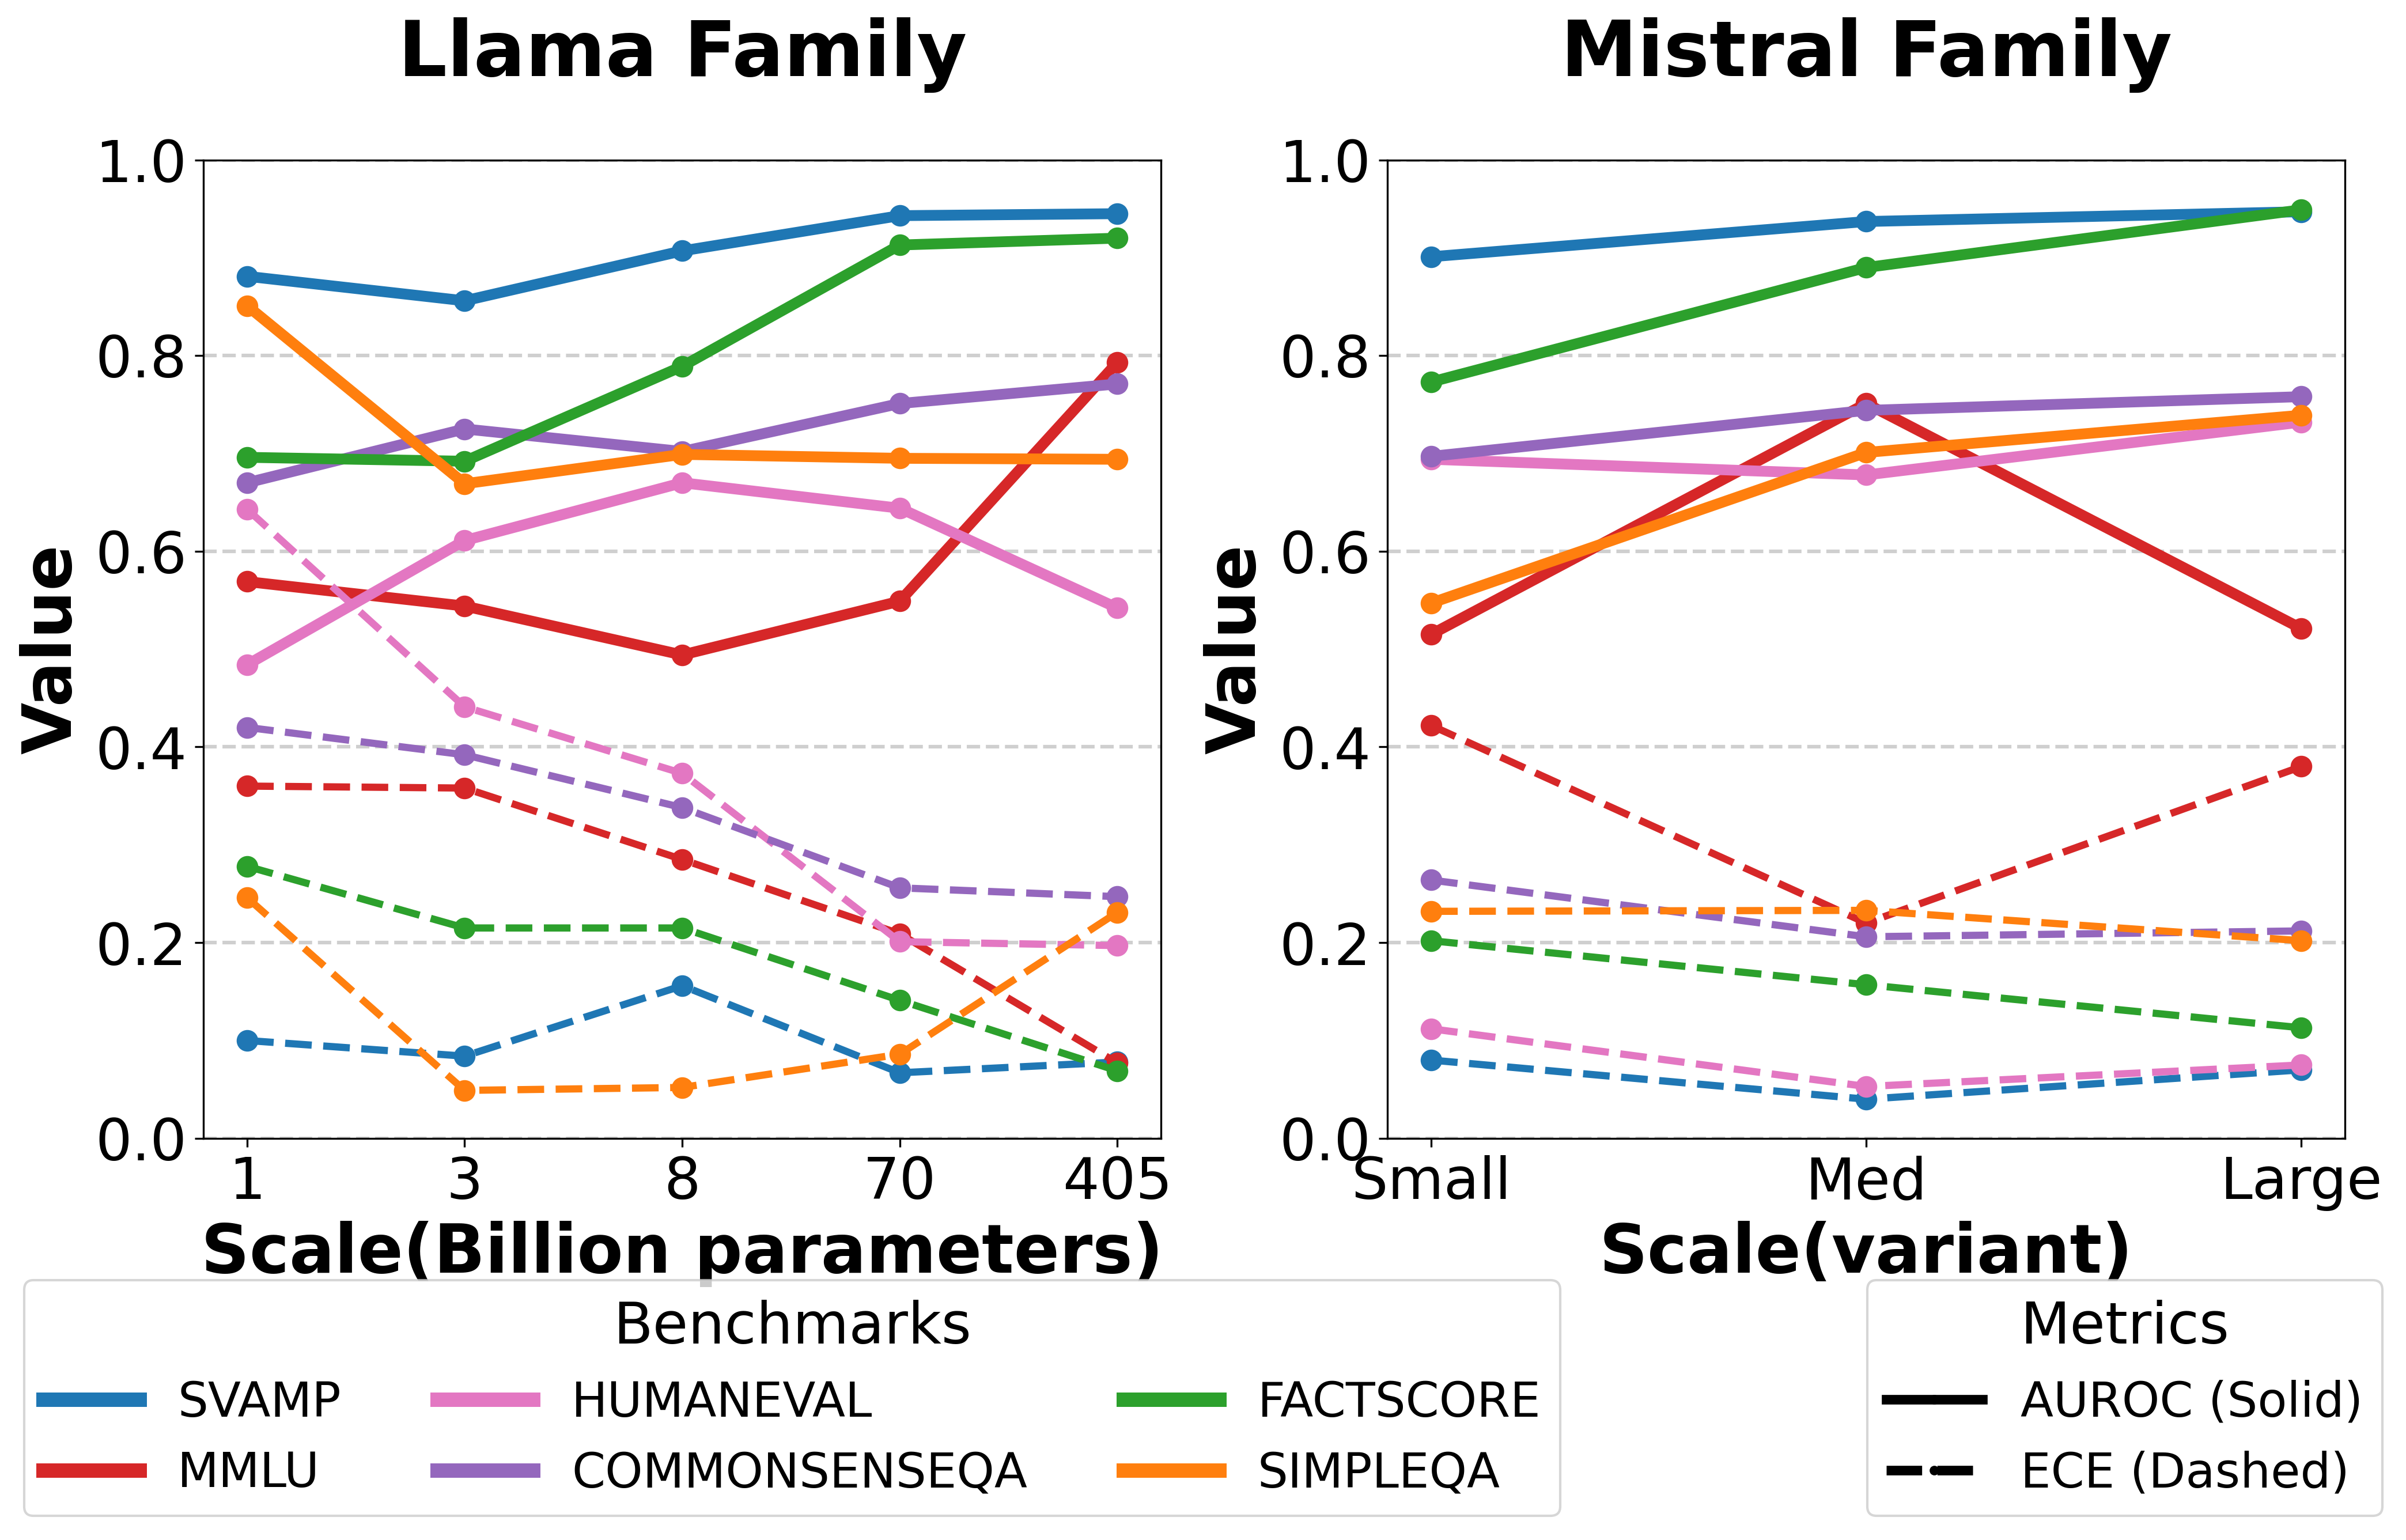
\includegraphics[width=\linewidth]{scaling_laws.png}
    \caption{\revised{Existing descriptive scaling comparison. Colors indicate benchmarks; solid lines show AUROC and dashed lines ECE. The plot does not isolate scale from model-family or training differences, and no significance claim is inferred from its visual trend.}}
    \label{fig:auroc_scaling_small_large_text}

\end{figure}

\begin{figure}[t]

    \centering
    \includegraphics[width=\linewidth]{alignment_Facuality.png}
    \caption{\revised{Existing aggregated factuality comparison on FActScore and SimpleQA. The source manuscript reports Spearman correlations of $0.624$ and $0.642$, and AUROC values of $0.831$ and $0.821$, respectively. These differ from the macro averages in Table~\ref{tab:main_results}; the exact aggregation pipeline must be reconciled before interpreting the difference.}}
    \label{fig:factuality}

\end{figure}

\end{document}
